%%%%%%%%%%%%%%%%%%%%%%%%%%%%%%%%%%%%%%%%%
% Masters/Doctoral Thesis 
% LaTeX Template
% Version 2.5 (27/8/17)
%
% This template was downloaded from:
% http://www.LaTeXTemplates.com
%
% Version 2.x major modifications by:
% Vel (vel@latextemplates.com)
%
% This template is based on a template by:
% Steve Gunn (http://users.ecs.soton.ac.uk/srg/softwaretools/document/templates/)
% Sunil Patel (http://www.sunilpatel.co.uk/thesis-template/)
%
% Template license:
% CC BY-NC-SA 3.0 (http://creativecommons.org/licenses/by-nc-sa/3.0/)
%
%%%%%%%%%%%%%%%%%%%%%%%%%%%%%%%%%%%%%%%%%

%----------------------------------------------------------------------------------------
%	PACKAGES AND OTHER DOCUMENT CONFIGURATIONS
%----------------------------------------------------------------------------------------

\documentclass[
11pt, % The default document font size, options: 10pt, 11pt, 12pt
%oneside, % Two side (alternating margins) for binding by default, uncomment to switch to one side
english, % ngerman for German
singlespacing, % Single line spacing, alternatives: onehalfspacing or doublespacing
%draft, % Uncomment to enable draft mode (no pictures, no links, overfull hboxes indicated)
%nolistspacing, % If the document is onehalfspacing or doublespacing, uncomment this to set spacing in lists to single
%liststotoc, % Uncomment to add the list of figures/tables/etc to the table of contents
%toctotoc, % Uncomment to add the main table of contents to the table of contents
%parskip, % Uncomment to add space between paragraphs
%nohyperref, % Uncomment to not load the hyperref package
headsepline, % Uncomment to get a line under the header
%chapterinoneline, % Uncomment to place the chapter title next to the number on one line
%consistentlayout, % Uncomment to change the layout of the declaration, abstract and acknowledgements pages to match the default layout
]{MastersDoctoralThesis} % The class file specifying the document structure

\usepackage[utf8]{inputenc} % Required for inputting international characters
\usepackage[T1]{fontenc} % Output font encoding for international characters
\usepackage{mathpazo} % Use the Palatino font by default
\usepackage{comment,import} 
\usepackage{booktabs,multicol,multirow,makecell,amsmath,afterpage}
\usepackage{tikz,tabularx,adjustbox}
\usepackage{subcaption}
\usetikzlibrary{shapes.geometric,matrix,arrows,positioning,calc,intersections}

\usepackage[colorlinks,bookmarksopen,bookmarksnumbered,citecolor=black,urlcolor=black]{hyperref}
\usepackage[backend=bibtex,style=numeric,natbib=true]{biblatex} % Use the bibtex backend with the authoryear citation style (which resembles APA)
\addbibresource{example.bib} % The filename of the bibliography
\usepackage[autostyle=true]{csquotes} % Required to generate language-dependent quotes in the bibliography


%----------------------------------------------------------------------------------------
%	MARGIN SETTINGS
%----------------------------------------------------------------------------------------

\geometry{
	paper=a4paper, % Change to letterpaper for US letter
	inner=2.5cm, % Inner margin
	outer=3.8cm, % Outer margin
	bindingoffset=.5cm, % Binding offset
	top=1.5cm, % Top margin
	bottom=1.5cm, % Bottom margin
	%showframe, % Uncomment to show how the type block is set on the page
}

%----------------------------------------------------------------------------------------
%	THESIS INFORMATION
%----------------------------------------------------------------------------------------

\thesistitle{Thesis Title} % Your thesis title, this is used in the title and abstract, print it elsewhere with \ttitle
\supervisor{Dr. James \textsc{Smith}} % Your supervisor's name, this is used in the title page, print it elsewhere with \supname
\examiner{} % Your examiner's name, this is not currently used anywhere in the template, print it elsewhere with \examname
\degree{Doctor of Philosophy} % Your degree name, this is used in the title page and abstract, print it elsewhere with \degreename
\author{John \textsc{Smith}} % Your name, this is used in the title page and abstract, print it elsewhere with \authorname
\addresses{} % Your address, this is not currently used anywhere in the template, print it elsewhere with \addressname

\subject{Biological Sciences} % Your subject area, this is not currently used anywhere in the template, print it elsewhere with \subjectname
\keywords{} % Keywords for your thesis, this is not currently used anywhere in the template, print it elsewhere with \keywordnames
\university{\href{http://www.university.com}{University Name}} % Your university's name and URL, this is used in the title page and abstract, print it elsewhere with \univname
\department{\href{http://department.university.com}{Department or School Name}} % Your department's name and URL, this is used in the title page and abstract, print it elsewhere with \deptname
\group{\href{http://researchgroup.university.com}{Research Group Name}} % Your research group's name and URL, this is used in the title page, print it elsewhere with \groupname
\faculty{\href{http://faculty.university.com}{Faculty Name}} % Your faculty's name and URL, this is used in the title page and abstract, print it elsewhere with \facname

\AtBeginDocument{
\hypersetup{pdftitle=\ttitle} % Set the PDF's title to your title
\hypersetup{pdfauthor=\authorname} % Set the PDF's author to your name
\hypersetup{pdfkeywords=\keywordnames} % Set the PDF's keywords to your keywords
}
\begin{document}

\frontmatter % Use roman page numbering style (i, ii, iii, iv...) for the pre-content pages

\pagestyle{plain} % Default to the plain heading style until the thesis style is called for the body content

%----------------------------------------------------------------------------------------
%	TITLE PAGE
%----------------------------------------------------------------------------------------

\begin{titlepage}
\begin{center}

\vspace*{.06\textheight}
{\scshape\LARGE \univname\par}\vspace{1.5cm} % University name
\textsc{\Large Doctoral Thesis}\\[0.5cm] % Thesis type

\HRule \\[0.4cm] % Horizontal line
{\huge \bfseries \ttitle\par}\vspace{0.4cm} % Thesis title
\HRule \\[1.5cm] % Horizontal line
 
\begin{minipage}[t]{0.4\textwidth}
\begin{flushleft} \large
\emph{Author:}\\
\href{http://www.johnsmith.com}{\authorname} % Author name - remove the \href bracket to remove the link
\end{flushleft}
\end{minipage}
\begin{minipage}[t]{0.4\textwidth}
\begin{flushright} \large
\emph{Supervisor:} \\
\href{http://www.jamessmith.com}{\supname} % Supervisor name - remove the \href bracket to remove the link  
\end{flushright}
\end{minipage}\\[3cm]
 
\vfill

\large \textit{A thesis submitted in fulfillment of the requirements\\ for the degree of \degreename}\\[0.3cm] % University requirement text
\textit{in the}\\[0.4cm]
\groupname\\\deptname\\[2cm] % Research group name and department name
 
\vfill

{\large \today}\\[4cm] % Date
%\includegraphics{Logo} % University/department logo - uncomment to place it
 
\vfill
\end{center}
\end{titlepage}

%----------------------------------------------------------------------------------------
%	DECLARATION PAGE
%----------------------------------------------------------------------------------------

\begin{declaration}
\addchaptertocentry{\authorshipname} % Add the declaration to the table of contents
\noindent I, \authorname, declare that this thesis titled, \enquote{\ttitle} and the work presented in it are my own. I confirm that:

\begin{itemize} 
\item This work was done wholly or mainly while in candidature for a research degree at this University.
\item Where any part of this thesis has previously been submitted for a degree or any other qualification at this University or any other institution, this has been clearly stated.
\item Where I have consulted the published work of others, this is always clearly attributed.
\item Where I have quoted from the work of others, the source is always given. With the exception of such quotations, this thesis is entirely my own work.
\item I have acknowledged all main sources of help.
\item Where the thesis is based on work done by myself jointly with others, I have made clear exactly what was done by others and what I have contributed myself.\\
\end{itemize}
 
\noindent Signed:\\
\rule[0.5em]{25em}{0.5pt} % This prints a line for the signature
 
\noindent Date:\\
\rule[0.5em]{25em}{0.5pt} % This prints a line to write the date
\end{declaration}

\cleardoublepage

%----------------------------------------------------------------------------------------
%	QUOTATION PAGE
%----------------------------------------------------------------------------------------

\vspace*{0.2\textheight}

\noindent\enquote{\itshape Thanks to my solid academic training, today I can write hundreds of words on virtually any topic without possessing a shred of information, which is how I got a good job in journalism.}\bigbreak

\hfill Dave Barry

%----------------------------------------------------------------------------------------
%	ABSTRACT PAGE
%----------------------------------------------------------------------------------------

\begin{abstract}
\addchaptertocentry{\abstractname} % Add the abstract to the table of contents
The main challenge presented by the laminated composite design is the laminate
layup, involving a set of fiber orientations, composite material systems, and
stacking sequences. In practice, it can be formulate as a constrained
combinatorial optimization problems which can be solved by the genetic
algorithm. However, genetic algorithm is invented for unconstrained problem,
which means to use this algorithm you need convert a constrained problem to an
unconstrained problem, for example, appending punishment items to the objective
function. 

In the present study,  a genetic algorithm methodological framework-based
optimization procedure is proposed for constrained problems 

minimize thickness(or weight) of
midplane-symmetric composite laminate subject to in-plane loading. Fiber
orientation and ply thickness are chosen as design variables, and a variant of GA is 
employed to search for the optimal design of composite laminates.  To avoid
spurious laminate designs, both the Tsai-wu and the maximum stress criteria are
taken to determine whether load-bearing capacity is exceeded or not. Numerical
results are obtained and presented under different loading cases.


In this present study, a new variant of
the genetic algorithm is proposed for the optimal design by modifying the
selection strategy.
To check the feasibility of a laminate subject to in-plane
loading, the effect of the fiber orientation angles and material components on
the first ply failure is studied. Then we compare the experimental results with
works in other literature.

Traditionally, classic lamination theory is widely used to compute
properties of composite materials under in-plane and out-of-plane loading from
a knowledge of the material properties of the individual layers and the
laminate geometry. In this study, a systematic procedure is proposed to design
an artificial neural network for a practical engineering problem, which is
applied to calculate the strength ratio of a laminated composite material under
in-plane loading, in which the genetic algorithm is proposed to optimize the search
process at four different levels: the architecture, parameters, connections of
the neural network, and active functions. 

\end{abstract}

%----------------------------------------------------------------------------------------
%	ACKNOWLEDGEMENTS
%----------------------------------------------------------------------------------------

\begin{acknowledgements}
\addchaptertocentry{\acknowledgementname} % Add the acknowledgements to the table of contents
The acknowledgments and the people to thank go here, don't forget to include your project advisor\ldots
\end{acknowledgements}

%----------------------------------------------------------------------------------------
%	LIST OF CONTENTS/FIGURES/TABLES PAGES
%----------------------------------------------------------------------------------------

\tableofcontents % Prints the main table of contents

\listoffigures % Prints the list of figures

\listoftables % Prints the list of tables

%%----------------------------------------------------------------------------------------
%	ABBREVIATIONS
%----------------------------------------------------------------------------------------

\begin{abbreviations}{ll} % Include a list of abbreviations (a table of two columns)

\textbf{LAH} & \textbf{L}ist \textbf{A}bbreviations \textbf{H}ere\\
\textbf{WSF} & \textbf{W}hat (it) \textbf{S}tands \textbf{F}or\\

\end{abbreviations}

%----------------------------------------------------------------------------------------
%	PHYSICAL CONSTANTS/OTHER DEFINITIONS
%----------------------------------------------------------------------------------------

\begin{constants}{lr@{${}={}$}l} % The list of physical constants is a three column table

% The \SI{}{} command is provided by the siunitx package, see its documentation for instructions on how to use it

Speed of Light & $c_{0}$ & \SI{2.99792458e8}{\meter\per\second} (exact)\\
%Constant Name & $Symbol$ & $Constant Value$ with units\\

\end{constants}

%----------------------------------------------------------------------------------------
%	SYMBOLS
%----------------------------------------------------------------------------------------

\begin{symbols}{lll} % Include a list of Symbols (a three column table)

$a$ & distance & \si{\meter} \\
$P$ & power & \si{\watt} (\si{\joule\per\second}) \\
%Symbol & Name & Unit \\

\addlinespace % Gap to separate the Roman symbols from the Greek

$\omega$ & angular frequency & \si{\radian} \\

\end{symbols}


%----------------------------------------------------------------------------------------
%	DEDICATION
%----------------------------------------------------------------------------------------

%\dedicatory{For/Dedicated to/To my\ldots} 

%----------------------------------------------------------------------------------------
%	THESIS CONTENT - CHAPTERS
%----------------------------------------------------------------------------------------

\mainmatter % Begin numeric (1,2,3...) page numbering

\pagestyle{thesis} % Return the page headers back to the "thesis" style

% Include the chapters of the thesis as separate files from the Chapters folder
% Uncomment the lines as you write the chapters

% Chapter Template

\chapter{Introduction} % Main chapter title

\label{Chapter1} % Change X to a consecutive number; for referencing this chapter elsewhere, use \ref{ChapterX}

%----------------------------------------------------------------------------------------
%	SECTION 1
%----------------------------------------------------------------------------------------

\section{Laminated Composite Material}

Composite materials offer improved strength, stiffness, corrosion resistance,
etc. over conventional materials, and are widely used as alternative materials
for applications in various industries ranging from electronic packaging to golf
clubs, and medical equipment to homebuilding, making aircraft structure to space
vechicles. The stacking sequence and fiber orientation of composite laminates
give the designer additional 'degree of freedom' to tailor the design with
respect to strength or stiffness.  One widely known advange of using composite
material is can significantly reducing the weight of target structure, and many
researchers attempted to improve the efficiency of using composite materail by
mimimizing the thickness.

Classic lamination theory(CLT) is used to develop the stress-strain relationship of
composite material under in-plane and out-of-plane loading. First, develop
stress-strain relationships, elastic moduli, strengths of an angle ply based on
a unidirectional lamina and the angle of the ply; second, becasue a laminate is
consist of more than one lamina bonded together through their thickness, so the
macromechianical analysis will be developed for a laminate based on applied
loading.  To check whether a designed lay-up is plausible or not, different
failure theories have been developed.

\section{Introduction}
Fiber-reinforced composite materials have been widely used in many industries
because they offer improved mechanical stiffness, strength, and low specific
gravity of fibers  over conventional materials. The use of composite material
materials in structural application is range from electronic packaging, sports
equipment, homebuilding, medical prosthetic devices, to high performance
military structures. The stacking sequence, ply thickness, and fiber
orientation of composite laminates give the designer additional ’degree of
freedom’ to tailor the design with respect to strength or stiffness. Classic
lamination theory(CLT) is taken to predict the behavior of a laminate from a
knowledge of the composite laminate properties of the individual layers and the
laminate geometry.

Evolutionary artificial neural networks(EANN's) is a special class of artifical
neural networks(ANN's) in which evolutionary algorithms(ES's) are introduced to
learn the optimal ANN. EA's can be used in the ANN at three different levels:
connection weights, architectures, input features, and learning rules. It is
shown, the combinations of ANN's and EA's can significantly improve the
performance of intelligent systems that rely's on ANN's or EA's alone.



The rest of the paper is organized as follows. Section 2 explains the classical
laminate theory and the failure criteria taken in the present study. Section 3
explains the design of artifical neural network for mathmatical model
approximation.  Section 4 reviews the use of genetic algorithm in the design of
neural network architecture and the parameters optimization during the training
process of neural network.  design Section 4 describes the result of the
numerical experiments in different cases, and in the Conclusion section we
dicuss the results.
\section{Classic Lamination Theory}
Classical lamination theory is based upon three simplifying engineering
assumptions: (1) Each layer's thickness is very small and consist of
homogeneous, orthotropic material, and these layers are prefectly bonded
together; (2) The entire laminated composite is supposed to be under plane
stress; (3) Normal cross sections of the entire laminate is normal to the
deflected middle surface, and do not change in thickness.
\begin{figure}
\centering
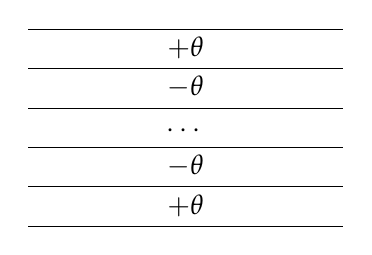
\begin{tikzpicture}
	\draw (0,0) -- (4,0);
	\draw (0,-0.5) -- (4,-0.5) node[midway, above] {$\mathit{+}\theta$};
	\draw (0,-1) -- (4,-1) node[midway, above] {$\mathit{-}\theta$} ;
	\draw (0,-1.5) -- (4,-1.5) node[midway, above] {$\cdots$};
	\draw (0,-2) -- (4,-2) node[midway, above] {$\mathit{-}\theta$};
	\draw (0,-2.5) -- (4,-2.5) node[midway, above] {$\mathit{+}\theta$};
\end{tikzpicture}
\caption{Model for Angle ply laminate}
\end{figure}

\subsection{Stress and Strain in a Lamina}
For a single lamina has a small thickness under plane stress, and it's upper and lower surfaces of the lamina are
free from external loads. According to the Hooke's Law, the three-dimensional stress-strain equations can be reduced to
two-dimensional stress-strain equations. The stress-strain relation in local axis 1-2 is:
\begin{equation}
    \begin{bmatrix}
        \sigma _1\\
        \sigma _2\\
        \tau_{12}
    \end{bmatrix}
    =
    \begin{bmatrix}
        Q_{11} & Q_{12} & 0\\
        Q_{12} & Q_{22} & 0\\
        0      &  0     & Q_{66}
    \end{bmatrix}
    \begin{bmatrix}
        \varepsilon_1\\
        \varepsilon_2\\\gamma_{12}
    \end{bmatrix}
\end{equation}
where $Q_{ij} $are the stiffnesses of the lamina that are related

to engineering elastic constants given by
\begin{equation}
    \begin{split}
    &Q_{11}=\frac{E_1}{1-v_{12}v_{21}}\\
    &Q_{22}=\frac{E_2}{1-v_{12}v_{21}}\\
    &Q_{66}=G_{12}\\
    &Q_{12}=\frac{v_{21}E_2}{1-v_{12}v_{21}}\\
    \end{split}
\end{equation}

where $E_1, E_2, v_{12}, G_{12} $ are four independent engineering elastic constants, which are defined as follows: $E_1 $ is the longitudinal Young's modulus, $E_2 $ is the transverse Young's modulus, $v_{12} $ is the major Poisson's ratio, and $G_{12} $ is the in-plane shear modulus.

Stress strain relation in the global x-y axis:
\begin{equation}
	\label{equ:stress-strain}
	\left[\begin{array}{l}
			\sigma _{x} \\ \sigma _{y} \\
			\tau_{xy}\end{array}\right]=\left[\begin{array}{lll}\bar{Q}_{11} &
			\bar{Q}_{12} & \bar{Q}_{16}\\ 
			\bar{Q}_{12} & \bar{Q}_{22} & \bar{Q}_{26} \\
								\bar{Q}_{16} & \bar{Q}_{26}
			 &\bar{Q}_{66}\end{array}\right]\left[\begin{array}{l}\varepsilon_{x}
	 \\ \varepsilon_{y}\\ \gamma_{x y}\end{array}\right] \end{equation}
where
\begin{equation}
	\begin{array}{l}
		\resizebox{.35\textwidth}{!}{$\bar{Q}_{11}=Q_{11} cos^{4}\theta+Q_{22} sin^{4}\theta+2\left(Q_{12}+2
		Q_{66}\right) sin^{2}\theta cos^{2}\theta$} \\

		\resizebox{.35\textwidth}{!}{$\bar{Q}_{12}=\left(Q_{11}+Q_{22}-4 Q_{66}\right) sin^{2}\theta
		cos^{2}\theta+Q_{12}\left(cos^{4}\theta+sin^{2}\theta \right)$} \\

		\resizebox{.35\textwidth}{!}{$\bar{Q}_{22}=Q_{11} sin^{4}\theta+Q_{22} cos^{4}\theta+2\left(Q_{12}+2
		Q_{66}\right) sin^{2}\theta cos^{2}\theta$} \\

		\resizebox{.4\textwidth}{!}{$\bar{Q}_{16}=\left(Q_{11}-Q_{12}-2
		Q_{66}\right) cos^{3}\theta sin\theta-\left(Q_{22}-Q_{12}-2Q_{66}\right)
	sin^{3}\theta cos\theta$} \\ 
		\resizebox{.4\textwidth}{!}{$\bar{Q}_{26}=\left(Q_{11}-Q_{12}-2
		Q_{66}\right) cos\theta sin^{3}\theta-\left(Q_{22}-Q_{12}-2
Q_{66}\right)cos^{3}\theta sin\theta$}
		 \\ 
	\resizebox{.4\textwidth}{!}	{$\bar{Q}_{66}=\left(Q_{11}+Q_{22}-2 Q_{12}-2 Q_{66}\right)
	sin\theta^{2}cos\theta^{2}+Q_{66}\left(sin\theta^{4}+cos\theta^{4}\right)$}\\
	\end{array}
\end{equation}



The local and global stresses in an angle lamina are related

to each other through the angle of the lamina $\theta $
\begin{equation}\left[\begin{array}{l}\sigma _{1} \\ \sigma _{2} \\ \tau_{12}\end{array}\right]=[T]\left[\begin{array}{l}\sigma _{x} \\ \sigma _{y} \\\tau_{xy}\end{array}\right]
\end{equation}

where
\begin{equation}
	[T]=\left[\begin{array}{ccc}cos^{2}\theta & sin^{2}\theta & 2
		sin\theta cos\theta \\ 
sin^{2}\theta & cos^{2}\theta & -2 sin\theta cos\theta \\
-sin\theta cos\theta
			  & sin\theta cos\theta  &cos^{2}\theta -sin^{2}\theta
\end{array}\right] 
\end{equation}



\subsection{Stress and Strain in a Laminate}
For forces and moment resultants acting on laminates, such as in plate and shell
structures, the relationship between applied forces and moment and displacement
can be given by

\begin{equation} \label{eq:force_and_moments}
	\begin{array}{l}
		\begin{aligned}
	\begin{bmatrix}
		N_x \\
		N_y \\
		N_{xy}
	\end{bmatrix}
	&=
	\begin{bmatrix}
		A_{11} & A_{12} & A_{16} \\
		A_{12} & A_{22} & A_{26} \\
		A_{16} & A_{26} & A_{66} 
	\end{bmatrix}
    \begin{bmatrix}
		\varepsilon_x^0 \\
        \varepsilon_y^0 \\
		\gamma_{xy}^0
    \end{bmatrix}   \\
	&+               
	\begin{bmatrix}
		B_{11} & B_{12} & B_{16} \\
		B_{11} & B_{12} & B_{16} \\
		B_{16} & B_{26} & B_{66} 
	\end{bmatrix}
	\begin{bmatrix}
		k_x \\
		k_y \\
		k_{xy} 
	\end{bmatrix}  \\
\end{aligned} \\ \\
\begin{aligned}
	\begin{bmatrix}
		M_x \\
		M_y \\
		M_{xy}
	\end{bmatrix}
	&=
	\begin{bmatrix}
		B_{11} & B_{12} & B_{16} \\
		B_{12} & B_{22} & B_{26} \\
		B_{16} & B_{26} & B_{66} 
	\end{bmatrix}
    \begin{bmatrix}
		\varepsilon_x^0 \\
        \varepsilon_y^0 \\
		\gamma_{xy}^0
    \end{bmatrix} \\ 
	&+  
	\begin{bmatrix}
		D_{11} & D_{12} & D_{16} \\
		D_{11} & D_{12} & D_{16} \\
		D_{16} & D_{26} & D_{66} 
	\end{bmatrix}
	\begin{bmatrix}
		k_x \\
		k_y \\
		k_{xy} 
	\end{bmatrix}
\end{aligned}
	\end{array}
\end{equation}


$N_x,N_y $  - normal force per unit length

$N_{xy} $  - shear force per unit length

$M_x, M_y $ - bending moment per unit length

$M_{xy} $  - twisting moments per unit length

$\varepsilon^{0}, k $- mid plane strains and curvature of a laminate in x-y coordinates

The mid plane strain and curvature is given by
\begin{equation}
    \begin{split}
    &A_{ij}=\sum_{k=1}^{n}(\overline{Q_{ij}})_k(h_k-h_{k-1})  i=1,2,6, j=1,2,6\\
    &B_{ij}=\frac{1}{2}\sum_{k=1}^{n}(\overline{Q_{ij}})_k(h_k^2 - h_{k-1}^2)  i=1,2,6, j=1,2,6\\
    &D_{ij}=\frac{1}{3}\sum_{k=1}^{n}(\overline{Q_{ij}})_k(h_k^3 - h_{k-1}^3) i=1,2,6, j=1,2,6\\
    \end{split}
\end{equation}

The [A], [B], and [D] matrices are called the extensional, coupling, and bending stiffness matrices,
respectively. The extensional stiffness matrix $[A]$ relates the resultant in-plane forces to the
in-plain strains, and the bending stiffness matrix $[D]$ couples the resultant bending moments to
the plane curvatures.  The coupling stiffness matrix $[B]$ relates the force and moment terms to the
midplain strains and midplane curvatures.

\section{Failure criteria for a lamina}

Failure criteria for composite materials are more difficult to predict due to
structural and material complexity in comparison to isotropic materials. The
failure process of a composite materials can be regarded from microscopic and
macroscopic points of view. Most popular criteria about the failure of an angle
lamina are in terms of macroscopic failure criteria, which are based on the
tensile, compressive and shear strengths. According to the failure surfaces,
these criteria
\cite{massard1984computer,reddy1987first,fang1993design,soeiro1994multilevel,pelletier2006multi,jadhav2007parametric,omkar2008artificial,choudhury2019failure},
can be classified into two classes: one is called independent failure mode
criteria which includes the maximum stress failure
theory\cite{watkins1987multicriteria}, maximum strain failure theory because
their failure envelop are rectangle; another is called quadratic polynomial
which includes Tsai-Wu\cite{martin1987optimum,soares1995discrete}, Chamis,
Hoffman and Hill criteria because their failure surfaces are of ellipsoidal
shape. In the present study, two most reliable failure criteria is taken,
Maximum stress and Tsai-wu.  Both of these two failure criteria are based on
the stresses in the local axes instead of principal normal stresses and maximum
shear stresses, and four normal strength parameters and one shear stress for a
unidirectional lamina are involved. The five strength parameters are

$(\sigma _1^{T})_{ult}= $ ultimate longitudinal tensile strength(in direction 1),

$(\sigma _1^{C})_{ult}= $ ultimate longitudinal compressive strength,

$(\sigma _2^{T})_{ult}= $ ultimate transverse tensile strength,

$(\sigma _2^{C})_{ult}= $ ultimate transverse compressive strength, and

$(\tau_{12})_{ult}= $ and ultimate in-plane shear strength.

\begin{figure}
\centering
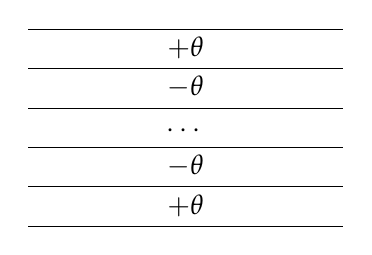
\begin{tikzpicture}
	\draw (0,0) -- (4,0);
	\draw (0,-0.5) -- (4,-0.5) node[midway, above] {$\mathit{+}\theta$};
	\draw (0,-1) -- (4,-1) node[midway, above] {$\mathit{-}\theta$} ;
	\draw (0,-1.5) -- (4,-1.5) node[midway, above] {$\cdots$};
	\draw (0,-2) -- (4,-2) node[midway, above] {$\mathit{-}\theta$};
	\draw (0,-2.5) -- (4,-2.5) node[midway, above] {$\mathit{+}\theta$};
\end{tikzpicture}
\caption{Model for Angle ply laminate}
\end{figure}


\subsection{Maximum stress failure criterion}(MS)


Maximum stress failure theory consists of maximum normal stress theory proposed by Rankine and maximum 
shearing stress theory by Tresca. The stresses applied on a lamina can be resolved into the normal and shear stresses 
in the local axes. If any of the normal or shear stresses in the local axes of a lamina is equal or exceeds the corresponding 
ultimate strengths of the unidirectional lamina, the lamina is considered to be failed. That is,

$\sigma_1 \geq (\sigma _1^{T})_{ult} $ or $\sigma_1 \leq -(\sigma _1^{C})_{ult} $

$\sigma_2 \geq (\sigma _2^{T})_{ult} $ or $\sigma_2 \leq -(\sigma _2^{C})_{ult} $

$\tau_{12} \geq (\tau_{12})_{ult} $  or $\tau_{12} \leq -(\tau_{12})_{ult} $

where $\sigma_1$ and $\sigma_2$ are the normal stresses in the local axes 1 and 2, respectively;
$\tau_{12}$ is the shear stress in the symmetry plane 1-2.

\subsection{Tsai-wu failure criterion}
The TW criterion is one of the most reliable static failure criteria which is derived from the von
Mises yield criterion.  
A lamina is considered to fail
if \begin{equation} \label{eq:tsai_wu}
\begin{split}
	H_1 \sigma_1  & + H_2 \sigma_2 + H_6 \tau_{12} + H_{11}\sigma_1^2 + H_{22} \sigma_2^2 \\
				  & + H_{66}  \tau_{12}^2 + 2H_{12}\sigma_1\sigma_2 < 1
\end{split}
\end{equation}

is violated, where

\begin{equation}
	\begin{split}
		H_{1}&=\frac{1}{\left(\sigma_{1}^{T}\right)_{u l t}}-\frac{1}{\left(\sigma_{1}^{C}\right)_{u l t}} \\
		H_{11}&=\frac{1}{\left(\sigma_{1}^{T}\right)_{u l t}\left(\sigma_{1}^{C}\right)_{u l t}} \\
		H_{2}&=\frac{1}{\left(\sigma_{2}^{T}\right)_{u l t}}-\frac{1}{\left(\sigma_{2}^{C}\right)_{u l t}} \\
		H_{22}&=\frac{1}{\left(\sigma_{2}^{T}\right)_{u l t}\left(\sigma_{2}^{C}\right)_{u l t}} \\
		H_{66}&=\frac{1}{\left(\tau_{12}\right)_{u l t}^{2}} \\
		H_{12}&=-\frac{1}{2} \sqrt{\frac{1}{\left(\sigma_{1}^{T}\right)_{u l
		t}\left(\sigma_{1}^{C}\right)_{u l t}\left(\sigma_{2}^{T}\right)_{u l
		t}\left(\sigma_{2}^{C}\right)_{u l t}}}
	\end{split}
\end{equation}

$H_i$ is the strength tensors of the second order; $H_{ij}$ is the strength
tensors of the fourth order. $\sigma_1$ is the applied normal stress in 
direction 1; $\sigma_2$ is the applied normal stress in the direction 2; and
$\tau_{12}$ is the applied in-plane shear stress.





\begin{figure}
\centering
\begin{tikzpicture}
	\begin{scope}
		%\draw[style=help lines] (-3,-3) grid (3,3);
		\draw (0,0) rectangle (2,3);
		\draw[->] (1.3,1.2) -- (2.6,1.2);
		\draw[->] (1.3,1.2) -- (1.3,3.4);
		\node at (2.2,1) {$X_T$};
		\node at (1.5, 3.2) {$Y_T$};
		\node at (-0.2, 0.9) {$X_C$};
		\node at (1.8, -0.2) {$Y_C$};
	\end{scope}
	\begin{scope}[xshift=6cm,yshift=1.15cm]
		%\draw[style=help lines] (-3,-3) grid (3,3);
		\draw[rotate=30] (0,0) ellipse (2cm and 1cm);
		\draw[->] (0.2,0) -- (0.2,2.2);
		\draw[->] (0.2,0) -- (1.9,0);
		\node at (1.6,-0.2) {$X_T$};
		\node at (0.3, 1.3) {$Y_T$};
		\node at (-1.6, 0) {$X_C$};
		\node at (-0.5, -1.5) {$Y_C$};
	\end{scope}
\end{tikzpicture}
\caption{Schematic failure surfaces for maximum stress and quadratic failure
criteria}
\end{figure}


\subsection{Failure Theories for a Laminate}
If keep increasing the loading applied to a laminate, the laminate will fails. The failure process
of a laminate is more complicate than a lamina, because a laminate consists of multiple plies, and
the fiber orientation, material, thickness of each ply maybe different from the others. In most
situations, some layer fails first and the remains continue to take more loads until all the plies
fail.  If one ply fails, it means this lamina does not contribute to the load carrying capacity of
the laminate. The procedure for finding the first failure ply given follows the fully discounted
method:

\begin{enumerate}
\item Compute the reduced stiffness matrix [Q] referred to as the local axis for each ply using its
	four engineering elastic constants $E_1 $, $E_2 $, $E_{12} $, and $G_{12} $.

\item Calculate the transformed reduced stiffness $[\bar{Q}] $ referring to the global coordinate
	system (x, y) using the reduced stiffness matrix [Q] obtained in step 1 and the ply angle for
	each layer.

\item  Given the thickness and location of each layer, the three laminate stiffness matrices [A],
	[B], and [D] are determined.

\item  Apply the forces and moments, $[N]_{xy}, [M]_{xy} $ solve Equation
	\ref{eq:force_and_moments}, and calculate the middle plane strain $[\sigma ^{0}]_{xy} $ and
	curvature $[k]_{xy} $.

\item Determine the local strain and stress of each layer under the applied load.

\item  Use the ply-by-ply stresses and strains in the Tsai-wu failure theory to find the strength
	ratio, and the layer with smallest strenght ratio is the first failed ply. 
\end{enumerate}

\subsection{Safety factor}
The safety factor, or yield stress, is how much extra load beyond is intended a
composite laminate will actually take. The safey factor is defined as 

\begin{equation} \label{eq:sr}S R=\frac{\text {Maximum Load Which Can Be Applied}}{\text {Load Applied}}
\end{equation}.

\subsection{Safety factor}
The safety factor, or yield stress, is how much extra load beyond is intended a
composite laminate will actually take, which is an indication of the material's
load carrying capacity. If the value is less then 1.0, it means failure. The safey factor is defined as 

\begin{equation} \label{eq:sr}S R=\frac{\text {Maximum Load Which Can Be Applied}}{\text {Load Applied}}
\end{equation}.

The safety factor based on maximum stress theory is calculated by the following
method: first, the principal stresses($\sigma_1^k$,$\sigma_2^k$, and
$\tau_{12}^k$) are obtained by experiment; evaluate the safety factor along each
direction according to equation \ref{eq:sr}; The minimum value among these
safety factors are denoted as the safety factor of the lamina, $SF_{MS}^k$.

\begin{align}
	SF_{MS}^k = \text{min of}
	\begin{cases}
		SF_X^k = 
		\begin{cases}
			\frac{X_t}{\sigma_{11}}, \text{ if } \sigma_{11}>0 \\
			\frac{X_c}{\sigma_{11}}, \text{ if } \sigma_{11}<0 \\
		\end{cases} \\
		SF_Y^k = 
		\begin{cases}
			\frac{Y_t}{\sigma_{22}}, \text{ if } \sigma_{22}>0 \\
			\frac{Y_c}{\sigma_{22}}, \text{ if } \sigma_{22}<0 \\
		\end{cases} \\
		SF_S^k =
		\begin{cases}
			\frac{S}{|\tau_{12}|} \\
		\end{cases} \\
	\end{cases}
\end{align}


Assuming the composite laminate under a in-plane loading f, the corresponding
stress on local stress in direction 1, local stress in direction 2, and shear
stress for the kth lamina are $\sigma_1 SF_{TW}^k$, $\sigma_2SF_{TW}^k$, and $\tau_{12}SF_{TW}^k$,
respectively. Substitute them into the equation \ref{eq:tsai_wu}, the expression
are given by

$a(SF_{TW}^k)^2 + b(SF_{TW}^k) - 1 = 0 $

where 

$a = H_{11}(\sigma_1)^2 + H_{22}(\sigma_2)^2 +H_{66}(\tau_{12})^2 +
2H_{12}\sigma_1 \sigma_2 $

$b = H_1\sigma_1 + H_2 \sigma_2 + H_6 \tau_{12}$

Solve the above equation, the safety factor for the kth lamina is 

$SF_{TW}^k = |\frac{-b+ \sqrt{b^2 + 4a}}{2a}|$.

Then, the minimum of $SF_{TW}^k$ is taken as the safety factor of the
laminate which is written as

$SF_{TW}= \text{ min of } SF_{TW}^k \text{ for } k=1,2,\cdots, m-1,m$ .





In the design of composite material, gradient based optimization techiques are
not appliable in this domain, because the design varaibles, such as fiber
orientation, layer thickness, number of layers etc. are discrete. Genetic
algorithm(GA) can be adopted in the optimization problem becasue it doesn't require
the gradient information. Moreover, the GA has been proved a reliable techique
and widely used in the design of composite material. 

CLT is an classic analytical approach to obtain the stress and stain of
composite material, the disadvantage of this method is quiet cubersome and in
which involves compliate matrix and integration operations. Artificial neural
network(ANN) has been proved a reliable tool in modelling various engineering
system in practice without solving tricky equations and making ideal
assumptions. In this thesis, the ANN is taken to approximate the numberic
results based on CLT and failure theory.

\section{Summary}

In this chapter, we review the classical lamination theory for the stress and
strain analysis in composite material, then related failure theories are
introduced to check whether a composite material would fail or not. In the
following chapters, the CLT would be used to calculate the stress and strain
under in-plane loading, it would also be used to generate the training data for
stress and strain approximation based on neural network; in order to design a
proper composite material, the failure theory are used to decide the feasibility
of composite design.

The rest of this thesis is as follows: in chapter two, we review the classic
lamination theory and related classic lamination theory, which are widely
adopted in the design of composite material; To design composite material, we
provide a new framework of genetic algorithm in chapter three; In chapter four,
this genetic algorith framework is implemented to guide the design of composite
material in two different cases; chapter five discusses about the application of
artificial neural network in composite material for approximating the evaluation
result based on classic lamination theory and failure theory.

In this thesis, first, we review the use of composite material in practice,
then, the CLT to calculate the stress and strain under certain loading, last,
the failure theories which are used to decide whether a composite material will
failure or not. Second, the stochastic algorith, GA, is studied and implemented
in the desgin of composite material, two different cases are studied in which GA
can be taken to obtain the optimal lay-up. At last, ANN is introduced to
approximate the evaluation result of CLT, the reason for adopting ANN is to
reduce the computation complexity based on CLT.


% Chapter Template

\chapter{Classic Lamination Theory and Failure Theory} % Main chapter title

\label{Chapter2} % Change X to a consecutive number; for referencing this chapter elsewhere, use \ref{ChapterX}

%----------------------------------------------------------------------------------------
%	SECTION 1
%----------------------------------------------------------------------------------------

\section{Classic Lamination Theory}


\section{Failure Theory}
\subsection{Tsai-wu Failure Theory}
\subsection{Maximum Stress Failure Theory}

 
% Chapter Template

\chapter{A New Genetic Algorithm Model for Constrained Problem} % Main chapter title

\label{Chapter3} % Change X to a consecutive number; for referencing this chapter elsewhere, use \ref{ChapterX}

%----------------------------------------------------------------------------------------
%	SECTION 1
%----------------------------------------------------------------------------------------

\section{Genetic Algorithm Framework}
GA is one of the most reliable stochastic algorithm, which has been widely used
in discrete variables optimization problems  \cite { schmit1973optimum,
	schmit1977optimum, fukunaga1991strength, soares1995discrete, le1995improved,
	jayatheertha1996application, wang1996optimum, adali1997minimum,
	correia1997higher, scares1997optimization, abu1998optimum, lombardi1998anti,
le1998design, sivakumar1998optimum, barakat1999use, richard2000reliability,
moita2000sensitivity, soremekun2001composite, walker2003technique,
di2003multiconstrained, kere2003using}. In practice, fiber orientations are
restricted to a finite set of angles, and ply thickness is a specific numeric
value. Because the design variables are not continueous, a gradient based
optimization procedure, such as gradient descent method, is not suitable to cope
with such problems. Moreover, gradient based optimization approach is very eazy
to get trapped in local minima, and many local optimum may exist in structural
optimization problems. A stochastic algorithm, such as GA, is able to deal with
optimization problems with discrete design variables. Besides, stochastic method
could escape from local optimum, and obtain global optimum. 

Although GA gains different advantages for solving discrete problems, many
disadvantages exists within this method. First, the optimization process of GA
parameters, such as the population size, parent population, mutation percentage,
etc., is very tedious; Second, the GA needs to evaluate the objective function
many times to acheive the optimization, and the computation cost is very high;
the last problem within GA is the premature convergence. GA consists of five
basic parts: the variable encoding method, selection scheme, crossover operator,
mutation operator, and how the constraints are handled. A typical GA process is
show in Figure \ref{GA:old_model}.

\begin{figure}
\centering
	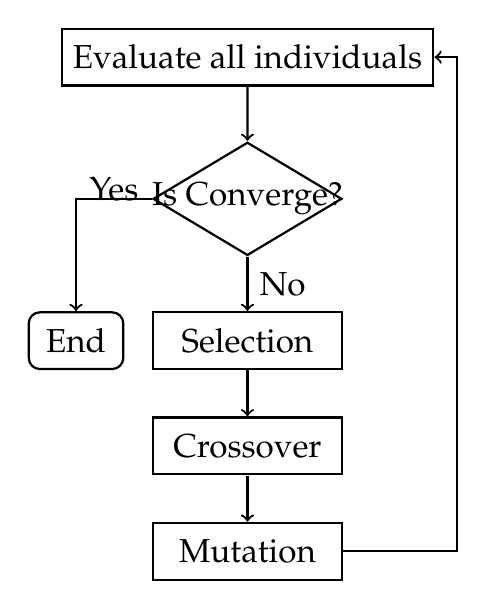
\begin{tikzpicture}[thick, scale=1.2, every node/.style={transform shape}]
		\tikzstyle{startstop} = [rectangle, rounded corners, minimum width=1.0cm,minimum height=0.6cm, text centered, draw=black]
		\tikzstyle{io} = [trapezium, trapezium left angle=70, trapezium right angle=110, minimum width=2cm, minimum height=0.6cm, text centered, draw=black]
		\tikzstyle{process} = [rectangle, minimum width=2cm, minimum height=0.6cm, text centered, draw=black]
		\tikzstyle{decision} = [diamond,minimum width=2cm, minimum height=1.2cm, draw=black]
		\node (fitness) [process] {Evaluate all individuals};
		\node[yshift=-0.5cm] (decision) [decision, below of=fitness] {} node at (decision.base) {Is Converge?};
		\node[yshift=-0.5cm] (selection) [process, below of=decision] {Selection};
		\node (crossover) [process] at ($(selection.south)+(0,-0.8cm)$) {Crossover};
		\node (mutation) [process] at ($(crossover.south)+(0,-0.8cm)$)  {Mutation};
		\node (end) [startstop] at ($(selection.west)+(-0.8cm,0cm)$) {End};

		\draw [->] (fitness) -- (decision);
		\draw [->] (decision.south) -- (selection.north) node[auto=left,pos=0.5]{No};
		\node at ($(decision.west)+(-0.4cm, 0.1cm)$) {Yes};
		\draw [->] (selection.south) -- (crossover.north);
		\draw [->] (crossover.south) -- (mutation.north);
		\draw [->] (decision.west) -| (end.north);
		\draw [->] (mutation.east) -- ($(mutation.east)+(1.2cm,0cm)$) |-
			(fitness.east);
	\end{tikzpicture}
\caption{Traditional GA Model.}
\label{fig:old_ga_model}
\end{figure}


The first issue when implementing a GA is the representation of design
variables, and an appropriate design representation is crucial to enhance the
efficiency of GA. The canonical GA has always used binary strings to encode
alternative solutions, however, some argued that the minimal cardinality, i.e.,
the binary representation, are not the best option. Real value string has been
widely employed in 

Selection scheme plays a critical role in balancing the dilemma of exploration
and exploitation inherented in GA, and various selection methods, for example,
roulette wheel, elitist, and tournament etc., have been proposed to overcome
this issue. Both of roulette selection and tournament selection are well-studied
and widely employed in the optimization design of laminated composite due to
their simplicity to code and efficiency for both nonparallel and parallel
architectures.

Crossover is another crucial operator introduced into the GA
methodology framework, in which the alternative solution is generated from the
mating pool.  multiple types of crossover operator has been utilized in the optimization
design of composite structures, such as: one-point, two-point, and uniform
crossover.
.

\section{Constrained Problem Optimization}
However, GA is originally proposed for unconstrained optimization problem, in
order to deal with constrained design for composite laminate, some techniques
are introduced into GA. The first method is using of data structure, special
data structure has been developed to fulfils the corresponding constraint, for
example, in order to fulfill the symmetry constraint of a laminate, the
chromsome is consist of coding only half of the laminate and considering that
each stack of the laminate is formed by two laminate with the same orientation
but opposite signs \cite{le1995improved,kogiso1994design}. The second approach
is reformulating the objective function.  A penalty function is developed to
convert a constrained problem into an unconstrained problem by adding penalty
term to the objective funtion. Another method to solve constrained problem is
introducing repair strategy by Todoroki and Haftka \cite{todoroki1998stacking},
which is aim to transform infeasible solutions to feasible solution by
incorporating problem-specific knowledge. 



%----------------------------------------------------------------------------------------
%	SECTION 2
%----------------------------------------------------------------------------------------
\section{A New Genetic Algorithm Model}

\begin{figure}
\begin{center}
	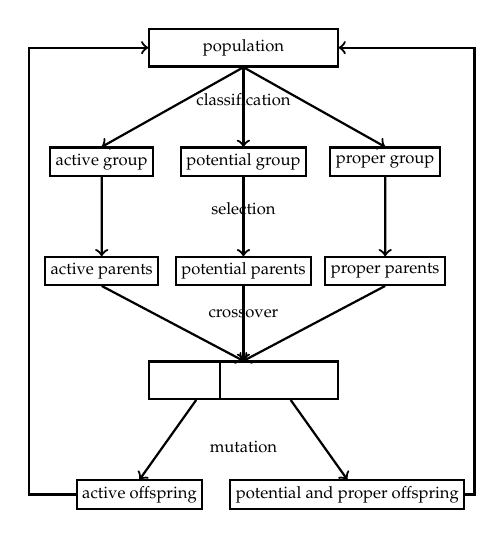
\begin{tikzpicture}[thick, scale=0.6, every node/.style={transform shape}]
	\tikzstyle{rec} = [rectangle, minimum width=4cm, minimum height=0.8cm,
	text centered, draw=black]
	\tikzstyle{subgroup} = [rectangle, minimum width=1.5cm, minimum height=0.6cm,
	text centered, draw=black]
	\tikzstyle{bigsubgroup} = [rectangle, minimum width=2.5cm, minimum height=0.6cm,
	text centered, draw=black]
	% population
	\node (population) [rec] {population};
	% active group
	\node (active_group_1) at ($(population.south)+(-3cm, -2.0cm)$) [subgroup]
		{active group};
	\node (active_group_2) at ($(active_group_1.south)+(0cm, -2.0cm)$)
		[subgroup] {active parents};
	\draw[->] (population.south) -- (active_group_1.north);
	\draw[->] (active_group_1.south) -- (active_group_2.north);
	% potential group
	\node (potential_group_1) at ($(population.south)+(0cm, -2.0cm)$) [subgroup]
		{potential group};
	\node (potential_group_2) at ($(potential_group_1.south)+(0cm, -2.0cm)$)
		[subgroup] {potential parents};
	\draw[->] (population.south) -- (potential_group_1.north);
	\draw[->] (potential_group_1.south) -- (potential_group_2.north);
	\node at ($(potential_group_1.north)+(0cm, 1.0cm)$) {classification };
	\node at ($(potential_group_2.north)+(0cm, 1.0cm)$) {selection};
    % proper group
	\node (proper_group_1) at ($(population.south)+(3cm, -2.0cm)$) [subgroup]
		{proper group};
	\node (proper_group_2) at ($(proper_group_1.south)+(0cm, -2.0cm)$)[subgroup]
		{proper parents};
	\draw[->] (population.south) -- (proper_group_1.north);
	\draw[->] (proper_group_1.south) -- (proper_group_2.north);
	% crossover
	\node (after_cross_over) at ($(potential_group_2.south)+(0cm, -2.0cm)$) [rec] {};
	\node  at ($(after_cross_over.north)+(0cm, 1.0cm)$)  {crossover};
	\draw[-] ($(after_cross_over.south)+(-0.5cm,0cm)$) --
		($(after_cross_over.north)+(-0.5cm,0cm)$);
	\draw[->] (active_group_2.south) -- (after_cross_over.north);
	\draw[->] (potential_group_2.south) -- (after_cross_over.north);
	\draw[->] (proper_group_2.south) -- (after_cross_over.north);
	% mutation
	\node (active_group_3) at ($(after_cross_over.south)+(-2.2cm, -2.0cm)$)
		[subgroup] {active offspring};
	\node at ($(after_cross_over.south)+(0cm, -1.0cm)$) {mutation};
	\draw[->] ($(after_cross_over.south)+(-1cm,0cm)$)--(active_group_3.north);
	\node (poteni_and_prop) at ($(after_cross_over.south)+(2.2cm, -2.0cm)$)
		[bigsubgroup] {potential and proper offspring};
	\draw[->] ($(after_cross_over.south)+(1cm,0cm)$)--(poteni_and_prop.north);

	% final draw
	\draw[->] (poteni_and_prop.east) --($(poteni_and_prop.east) + (0.2cm,0cm)$) |- (population.east);
	\draw[->] (active_group_3.west) -- ($(active_group_3.west) + (-1cm,0cm)$)
		|- (population.west);
\end{tikzpicture}
\end{center}
\caption{GA Model\label{GA:model}}
\end{figure}


\subsection{Classification}
The population is randomly generated, for every individual in this population
the corresponding constraint numberic value can be obtained. As shown in
Figure \ref{GA:model},The population can
be divided into three groups according to constraint value, which are active
group, potential group and proper group

\subsection{Selection}
The purpose of the selection operator is to chose mating pool to produce
alternative solutions of better fitness. Traditional methods of selecting
strategies only take the fitness of individuals into acount, however, due to 
the existance of constraint, various selection schemes are implemented to
selecet the mating set. Based on different selection schemes, the parents of
next generation can be divided into  three groups: proper groups, active groups,
and potential groups according to different selecting methods. 

Proper parents mean in which individual fullfils the constraints, which are
chosen by the individual's fitnees, individuals with better fitness are more
likely to be chosen if they fit the constraint; active groups means that
individual is supposed to be always exist in the parents during the GA, which
are selected by fitness, ignoring the constraint; The individuals from active
group may not correspond to feasible solutions, but their existance enriches the
variety of the gene clips.  Potential groups means that they are likely to turn
into proper individual after a couple of generations, and potential individuals
are chosen by constraint function, the more the individual fulfils the
constraint, the more possiblity it will be selected.

\subsection{Crossover}
The crossover operator happens among these three groups. the child of two proper
groups are more likely to be a proper individual which can be used to obtain a
alternative feasible solution. the child of an active individual and a potential
individual can significantly change the gene of active individual's chromsome,
which makes the individual evolve toward a new direction. The offspring of two
active individuals are more likely to be an active individual, which can maitain
the active group.  The figure.\ref{GA:operator} (b) shows two children $O_1$

\subsection{Mutation}
i


\section{Summary}
In this chapter, frist, we review the application of tradional GA in the design
of composite material; then A new GA framework has been come up with, in the
following chapters, this NGAM will be adopted to directed the lay-up design of
composite material.


% Chapter Template

\chapter{The Application of Artificial Neural Network in Composite Material} % Main chapter title

\label{Chapter4} % Change X to a consecutive number; for referencing this chapter elsewhere, use \ref{ChapterX}

%----------------------------------------------------------------------------------------
%	SECTION 1
%----------------------------------------------------------------------------------------


\section{Introduction}
Fiber-reinforced composite materials have been widely used in a variety of
applications, which include electronic packaging, sports equipment,
homebuilding, medical prosthetic devices, high-performance military
structures, etc. because they offer improved mechanical stiffness, strength,
and low specific gravity of fibers over conventional materials.  The stacking
sequence, ply thickness, and fiber orientation of composite laminates give the
designer an additional ’degree of freedom’ to tailor the design with respect to
strength or stiffness. CLT and failure theory, e.g., Tsai-Wu failure criteria,
is usually taken to predict the behavior of a laminate from a knowledge of the
composite laminate properties of the individual layers and the laminate
geometry.

However, the use of CLT needs intensive computation which takes an analytical
method to solve the problem, since it involves massive matrix multiplication
and integration calculation. Techniques of function approximation can
accelerate the calculation process and reduce the computation cost.  Artificial
neural network(ANN), heavily inspired by biology and psychology, is a reliable
tool instead of a complicated mathematical model. ANN has been widely used to
solve various practical engineering problems in applications, such as pattern
recognition, nonlinear regression, data mining, clustering,  prediction, etc.
Evolutionary artificial neural networks(EANNs) is a special class of
artificial neural networks, in which evolutionary algorithms are
introduced to design the topology of an ANN, and can be used at four different
levels: connection weights, architectures, input features, and learning rules.
It is shown that the combinations of ANN's and EA's can significantly improve
the performance of intelligent systems than that rely's on ANN's or
evolutionary algorithms alone.

The rest of this paper is organized as the following: section II introduces the
CLT and the failure criteria, which is used to check whether the composite
material fails or not in the present study; section III covers the design of
artificial neural network for a function approximation; section IV reviews the
use of the genetic algorithm in the design of neural network architecture, and
the techniques of parameters optimization during the training process; section
V presents the result of the numerical experiments in different cases; in the
conclusion part, we present and discuss the experiment results.





%\section{classical lamination theory and failure criteria}

\subsection{Classical Lamination Theory}


Classical lamination theory derives from three simplifying assumptions in
laminated composite material: the laminate consist of plies bonded together
through the thickness, the thickness of each ply is small, and it is consists of
homogeneous, orthotropic material; the entire laminated composite is only under
in-plane loading; the Normal cross-section of the laminate is vertical to the
deflected middle surface. Fig. \ref{fig:lamina_local_and_global} shows the
coordinate system used for an angle lamina. The axis in the 1-2 coordinate
system is called the local axis or the material axis, and the axis in the x-y
coordinate system is called the global axis.

\begin{figure}[b]
	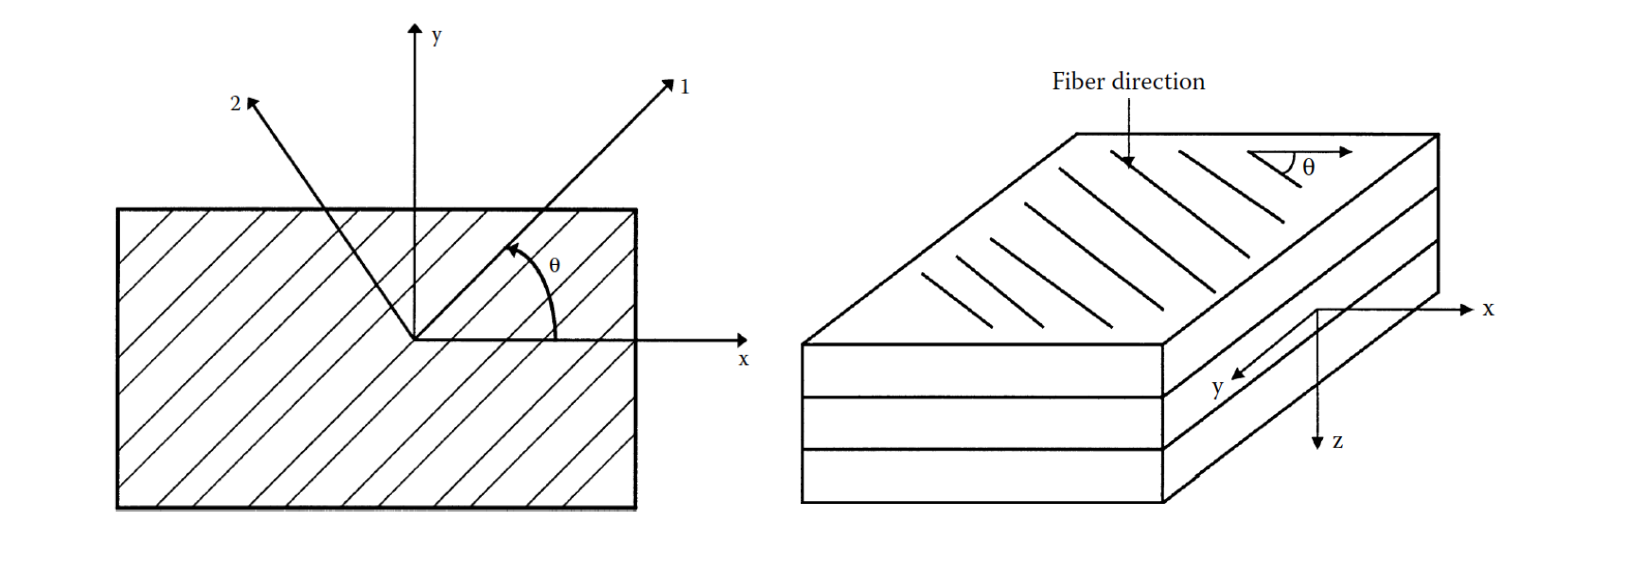
\includegraphics[width=1\linewidth]{fig/lamina_local_global_axes.png}
	\caption{The left diagram shows the local and global axis of an angle lamina, which is from a laminate as shown in the right diagram.}
	\label{fig:lamina_local_and_global}
\end{figure}

A few cases of laminates, such as symmetric laminates, cross-ply laminates, play
an important role in the application of laminated composite material. A laminate
is called an angle ply laminate if it has plies of the same material and
thickness and is only oriented at $+\theta$ and $-\theta$ directions. A model of
an angle ply laminate is as shown in Fig. \ref{fig:angle-ply}.

\begin{figure}[b]
\centering
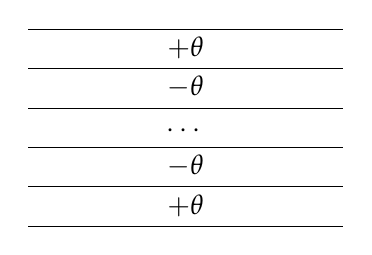
\begin{tikzpicture}
	\draw (0,0) -- (4,0);
	\draw (0,-0.5) -- (4,-0.5) node[midway, above] {$\mathit{+}\theta$};
	\draw (0,-1) -- (4,-1) node[midway, above] {$\mathit{-}\theta$} ;
	\draw (0,-1.5) -- (4,-1.5) node[midway, above] {$\cdots$};
	\draw (0,-2) -- (4,-2) node[midway, above] {$\mathit{-}\theta$};
	\draw (0,-2.5) -- (4,-2.5) node[midway, above] {$\mathit{+}\theta$};
\end{tikzpicture}
\caption{Model for angle ply laminate}
\label{fig:angle-ply}
\end{figure}


\subsubsection{Stress and Strain in a Lamina}
For a single lamina under in-plane loading whose thickness is relatively small,
suppose the upper and lower surfaces of the lamina are free from external
loading. According to Hooke's law, the three-dimensional stress-strain
equations can be reduced to two-dimensional stress-strain equations in the
composite material. The stress-strain relation in local axis 1-2 is
\begin{equation}
	\left[
		\begin{array}{l}
        	\sigma _1\\
        	\sigma _2\\
        	\tau_{12}
    	\end{array}
	\right]
    =
	\left[
		\begin{array}{ccc}
        	Q_{11} & Q_{12} & 0\\
        	Q_{12} & Q_{22} & 0\\
        	0      & 0     & Q_{66}
    	\end{array}
	\right]
	\left[
		\begin{array}{l}
        	\varepsilon_1\\
        	\varepsilon_2\\
			\gamma_{12}
		\end{array} 
	\right]\textstyle{,}
\end{equation}
where $Q_{ij} $ is the stiffness of a lamina. And they are related to
engineering elastic constants as follows:
\begin{equation}
	\begin{array}{l}
		Q_{11}=\frac{E_1}{1-v_{12}v_{21}} \textstyle{,} \\
    	Q_{22}=\frac{E_2}{1-v_{12}v_{21}} \textstyle{,}\\
    	Q_{66}=G_{12} \textstyle{,}\\
    	Q_{12}=\frac{v_{21}E_2}{1-v_{12}v_{21}} \textstyle{,}
    \end{array}
\end{equation}
where $E_1, E_2, v_{12}, G_{12} $ are four independent engineering elastic
constants, which are defined as follows: $E_1 $ is the longitudinal Young's
modulus, $E_2 $ is the transverse Young's modulus, $v_{12} $ is the major
Poisson's ratio, and $G_{12} $ is the in-plane shear modulus.

Stress-strain relation in the global x-y axis is
\begin{equation}
	\label{equ:stress-strain}
	\left[\begin{array}{l}
			\sigma _{x} \\ 
			\sigma _{y} \\
			\tau_{xy}
			\end{array}
	\right]=
	\left[\begin{array}{lll}
			\bar{Q}_{11} & \bar{Q}_{12} & \bar{Q}_{16}\\ 
			\bar{Q}_{12} & \bar{Q}_{22} & \bar{Q}_{26} \\
			\bar{Q}_{16} & \bar{Q}_{26} &\bar{Q}_{66}
		\end{array}
	 \right]
	 \left[\begin{array}{l}
			 \varepsilon_{x} \\ 
	 		 \varepsilon_{y} \\ 
	 		 \gamma_{x y}
	 		\end{array}
	\right] \textstyle{,}
\end{equation}
where
\begin{equation}
	\begin{array}{l}
		\resizebox{.35\textwidth}{!}{$\bar{Q}_{11}=Q_{11} cos^{4}\theta+Q_{22} sin^{4}\theta+2\left(Q_{12}+2
		Q_{66}\right) sin^{2}\theta cos^{2}\theta$}\textstyle{,} \\
		\resizebox{.35\textwidth}{!}{$\bar{Q}_{12}=\left(Q_{11}+Q_{22}-4 Q_{66}\right) sin^{2}\theta
			cos^{2}\theta+Q_{12}\left(cos^{4}\theta+sin^{2}\theta \right)$} \textstyle{,}\\
		\resizebox{.35\textwidth}{!}{$\bar{Q}_{22}=Q_{11} sin^{4}\theta+Q_{22} cos^{4}\theta+2\left(Q_{12}+2
				Q_{66}\right) sin^{2}\theta cos^{2}\theta$}\textstyle{,} \\
		\resizebox{.40\textwidth}{!}{$\bar{Q}_{16}=\left(Q_{11}-Q_{12}-2
			Q_{66}\right) cos^{3}\theta
			sin\theta-\left(Q_{22}-Q_{12}-2Q_{66}\right) sin^{3}\theta cos\theta$} \textstyle{,}\\ 
		\resizebox{.40\textwidth}{!}{$\bar{Q}_{26}=\left(Q_{11}-Q_{12}-2
			Q_{66}\right) cos\theta sin^{3}\theta-\left(Q_{22}-Q_{12}-2
			Q_{66}\right)cos^{3}\theta sin\theta$} \textstyle{,}\\ 
		\resizebox{.40\textwidth}{!}	{$\bar{Q}_{66}=\left(Q_{11}+Q_{22}-2 Q_{12}-2 Q_{66}\right)
			sin\theta^{2}cos\theta^{2}+Q_{66}\left(sin\theta^{4}+cos\theta^{4}\right)$}\textstyle{.}\\
	\end{array}
\end{equation}

\subsubsection{Stress and Strain in a Laminate}
For forces acting on laminates, such as in plate and shell
structures, the relationship between applied forces and displacement
can be given by

\begin{equation} \label{eq:force_and_moments}
	\begin{array}{ll}
	\begin{bmatrix}
		N_x \\
		N_y \\
		N_{xy}
	\end{bmatrix}
	&=
	\begin{bmatrix}
		A_{11} & A_{12} & A_{16} \\
		A_{12} & A_{22} & A_{26} \\
		A_{16} & A_{26} & A_{66} 
	\end{bmatrix}
    \begin{bmatrix}
		\varepsilon_x^0 \\
        \varepsilon_y^0 \\
		\gamma_{xy}^0
    \end{bmatrix}   \\
	&+               
	\begin{bmatrix}
		B_{11} & B_{12} & B_{16} \\
		B_{11} & B_{12} & B_{16} \\
		B_{16} & B_{26} & B_{66} 
	\end{bmatrix}
	\begin{bmatrix}
		k_x \\
		k_y \\
		k_{xy} 
	\end{bmatrix}  \textstyle{,}
	\end{array}
\end{equation}
where $N_x,N_y $ refers to the normal force per unit length;
$N_{xy}$ means shear force per unit length;
$\varepsilon^{0}$ and $k_{xy}$ denotes  mid plane strains and curvature of a laminate in x-y coordinates
The mid-plane strain and curvature is given by
\begin{equation}
    \begin{split}
	&A_{ij}=\sum_{k=1}^{n}(\overline{Q_{ij}})_k(h_k-h_{k-1})  i=1,2,6, j=1,2,6 \textstyle{,}\\
    &B_{ij}=\frac{1}{2}\sum_{k=1}^{n}(\overline{Q_{ij}})_k(h_k^2 - h_{k-1}^2)  i=1,2,6, j=1,2,6\textstyle{,}\\
    &D_{ij}=\frac{1}{3}\sum_{k=1}^{n}(\overline{Q_{ij}})_k(h_k^3 - h_{k-1}^3) i=1,2,6, j=1,2,6\textstyle{.}\\
    \end{split}
\end{equation}

The [A], [B], and [D] matrices are called the extensional, coupling, and bending stiffness matrices,
respectively. The extensional stiffness matrix $[A]$ relates the resultant in-plane forces to the
in-plain strains, and the bending stiffness matrix $[D]$ couples the resultant bending moments to
the plane curvatures.  The coupling stiffness matrix $[B]$ relates the force and moment terms to the
midplane strains and curvatures.

\subsection{Failure criteria for a lamina}

Failure criteria for composite materials are more difficult to predict due to
structural and material complexity. The failure process of composite materials
can be regarded from microscopic and macroscopic points of view. The most
popular criteria about the failure of an angle lamina are from the macroscopic
point of view, which are according to the tensile, compressive, and shear
strengths. As shown in Fig. \ref{fig:failure_surface}, there are two types of failure
criteria\cite{massard1984computer,reddy1987first,fang1993design,soeiro1994multilevel,pelletier2006multi,jadhav2007parametric,omkar2008artificial,choudhury2019failure}
according to failure surfaces. The first failure surface is a rectangle that
includes the maximum stress failure criterion\cite{watkins1987multicriteria},
and maximum strain failure criterion. The second failure surface is ellipsoidal
that includes Tsai-Wu\cite{martin1987optimum,soares1995discrete}, Chamis,
Hoffman, and Hill criteria. In the present study, the two most reliable failure
criteria are adopted, Maximum stress and Tsai-wu. Both these failure criteria
are based on the stress in the local axis instead of principal normal stress and
maximum shear stresses, in which four normal strength parameters and one shear
stress are involved. The five strength parameters are

$(\sigma _1^{T})_{ult}= $ ultimate longitudinal tensile strength(in direction 1),

$(\sigma _1^{C})_{ult}= $ ultimate longitudinal compressive strength,

$(\sigma _2^{T})_{ult}= $ ultimate transverse tensile strength,

$(\sigma _2^{C})_{ult}= $ ultimate transverse compressive strength, and

$(\tau_{12})_{ult}= $ and ultimate in-plane shear strength.

\begin{figure}[b]
\centering
\begin{tikzpicture}
	\begin{scope}
		%\draw[style=help lines] (-3,-3) grid (3,3);
		\draw (0,0) rectangle (2,3);
		\draw[->] (1.3,1.2) -- (2.6,1.2);
		\draw[->] (1.3,1.2) -- (1.3,3.4);
		\node at (2.2,1) {$X_T$};
		\node at (1.5, 3.2) {$Y_T$};
		\node at (-0.2, 0.9) {$X_C$};
		\node at (1.8, -0.2) {$Y_C$};
	\end{scope}
	\begin{scope}[xshift=6cm,yshift=1.15cm]
		%\draw[style=help lines] (-3,-3) grid (3,3);
		\draw[rotate=30] (0,0) ellipse (2cm and 1cm);
		\draw[->] (0.2,0) -- (0.2,2.2);
		\draw[->] (0.2,0) -- (1.9,0);
		\node at (1.6,-0.2) {$X_T$};
		\node at (0.3, 1.3) {$Y_T$};
		\node at (-1.6, 0) {$X_C$};
		\node at (-0.5, -1.5) {$Y_C$};
	\end{scope}
\end{tikzpicture}
\caption{Schematic failure surfaces for maximum stress and quadratic failure
criteria}
\label{fig:failure_surface}
\end{figure}

\subsubsection{Maximum stress(MS) failure criterion}

Maximum stress failure criteria are consist of the normal stress theory and the
shear stress theory. The stress applied to a lamina can be resolved into the
normal stress and shear stress in the local axis. The lamina fails if either of
the normal stress or shear stress in the local axis of a lamina is equal or
exceeds the corresponding ultimate strengths of the unidirectional lamina.  That
is,

\begin{equation}
	\begin{array}{lll}
		\sigma_1 \geq (\sigma _1^{T})_{ult} & \textstyle{ or } &  \sigma_1 \leq -(\sigma _1^{C})_{ult} \textstyle{,} \\
		\sigma_2 \geq (\sigma _2^{T})_{ult} & \textstyle{ or } &   \sigma_2 \leq -(\sigma _2^{C})_{ult} \textstyle{,} \\
		\tau_{12} \geq (\tau_{12})_{ult}    & \textstyle{ or } &     \tau_{12} \leq -(\tau_{12})_{ult}  \textstyle{,}
\end{array}
\end{equation}

where $\sigma_1$ and $\sigma_2$ are the normal stresses in the local axis 1 and 2;
$\tau_{12}$ is the shear stress in the symmetry plane 1-2.

\subsubsection{Tsai-Wu failure criterion}
The Tsai-Wu criterion is one of the most reliable static failure criteria derived from the von
Mises yield criterion.  
A lamina is considered to fail
if \begin{equation} \label{eq:tsai_wu}
\begin{split}
	H_1 \sigma_1  & + H_2 \sigma_2 + H_6 \tau_{12} + H_{11}\sigma_1^2 + H_{22} \sigma_2^2 \\
				  & + H_{66}  \tau_{12}^2 + 2H_{12}\sigma_1\sigma_2 < 1
\end{split}
\end{equation}

is violated, where

\begin{equation}
	\begin{split}
		H_{1}&=\frac{1}{\left(\sigma_{1}^{T}\right)_{u l t}}-\frac{1}{\left(\sigma_{1}^{C}\right)_{u l t}}\textstyle{,} \\
		H_{11}&=\frac{1}{\left(\sigma_{1}^{T}\right)_{u l t}\left(\sigma_{1}^{C}\right)_{u l t}} \textstyle{,}\\
		H_{2}&=\frac{1}{\left(\sigma_{2}^{T}\right)_{u l t}}-\frac{1}{\left(\sigma_{2}^{C}\right)_{u l t}} \textstyle{,}\\
		H_{22}&=\frac{1}{\left(\sigma_{2}^{T}\right)_{u l t}\left(\sigma_{2}^{C}\right)_{u l t}} \textstyle{,}\\
		H_{66}&=\frac{1}{\left(\tau_{12}\right)_{u l t}^{2}} \textstyle{,}\\
		H_{12}&=-\frac{1}{2} \sqrt{\frac{1}{\left(\sigma_{1}^{T}\right)_{u l
		t}\left(\sigma_{1}^{C}\right)_{u l t}\left(\sigma_{2}^{T}\right)_{u l
		t}\left(\sigma_{2}^{C}\right)_{u l t}}}\textstyle{.}
	\end{split}
\end{equation}

$H_i$ is the strength tensor of the second-order; $H_{ij}$ is the strength
tensor of the fourth-order. $\sigma_1$ is the applied normal stress in 
direction 1; $\sigma_2$ is the applied normal stress in direction 2; 
$\tau_{12}$ is the applied in-plane shear stress.




\subsubsection{Strength ratio}
The safety factor, or yield stress, is how much extra load beyond is intended a
composite laminate will take. The strength ratio(SR) is defined as 

\begin{equation}
	\label{eq:sr}S R=\frac{\text {Maximum Load Which Can Be Applied}}{\text {Load Applied}}\textstyle{.}
\end{equation}

\section{Evolutionary Artificial Neural Network}
\begin{figure}[tb]
\centering
	%\resizebox{.7\linewidth}{!}{dd
%\begin{tikzpicture}[show background grid, show background rectangle]
\begin{tikzpicture}
	\useasboundingbox (-3.5,-5.) rectangle (3.5,6.3);
	\scope[transform canvas={scale=1}]
    %\draw[help lines] (-3cm,-7cm) grid (6cm, 5cm);
    \tikzstyle{block} = [rectangle, text centered, draw=black,
    minimum width=1.1cm, minimum height=0.4cm]
	% first level evolution: connection weights
    \node (evaluation-parent) [block, minimum width=2.4cm, minimum
        height=1.8cm,draw=white] {};
    \node (evaluation) [block] at ($(evaluation-parent.north)$) {evaluation};
    \node (reproduction) [block] at ($(evaluation-parent.south)$) {reproduction};
    \node (tasks) [block, minimum width=1.1cm, minimum height=0.4cm] {tasks};

    \draw[->] ($(evaluation.south)+(0.3cm,0cm)$) --
        ($(tasks.north)+(0.3cm,0cm)$) node[auto=left, pos=0.5] {\small weights}; 
    \draw[<-] ($(evaluation.south)+(-0.3cm,0cm)$) --
        ($(tasks.north)+(-0.3cm,0cm)$) node[auto=right, pos=0.5] {\small fitness}; 

	\draw[black] (reproduction.west) -- ++(-0.3cm,0)  |- (evaluation.west);
	\draw[black] (reproduction.east) -- ++(0.3cm,0)   |- (evaluation.east);

    \node (level1) [block,draw=black, minimum width=3.5cm, minimum height=3.0cm] at
        (0cm,0.2cm) {};
    \node [align=left] at ($(level1.north)+(0,-0.2cm)$) {\tiny THE EVOLUTION
        OF};
    \node [align=left] at ($(level1.north)+(0,-0.45cm)$) {\tiny CONNECTION
            WEIGHTS
        };
    % second level evolution: active functions
    \node (level2_container) [block, draw=black, minimum width=5.8cm, minimum
        height=6.0cm] at
        (0, 0.4cm)  {};
    \node [align=left] at ($(level2_container.north)+(0,-0.25cm)$) {\tiny THE EVOLUTION
        OF ACTIVE FUNCTIONS};
    \node (level2-assister) [block, draw=white, minimum width=5cm, minimum
		height=4.6cm] at
        (0, 0.3cm)  {};
    \node (evaluation) [block] at ($(level2-assister.north)$) {\small evaluation of
        active functions};
    \node (reproduction) [block] at ($(level2-assister.south)$) {\small reproduction of
        active functions};

    \draw[->] ($(evaluation.south)+(0.3cm,0cm)$) --
        ($(level1.north)+(0.3cm,0cm)$) node[auto=left, pos=0.5] {\small active functions
        }; 

    \draw[<-] ($(evaluation.south)+(-0.3cm,0cm)$) --
        ($(level1.north)+(-0.3cm,0cm)$) node[auto=right, pos=0.5] {\small fitness}; 

	\draw[black] (reproduction.west) -- ++(-0.3cm,0)  |- (evaluation.west);
	\draw[black] (reproduction.east) -- ++(0.3cm,0)   |- (evaluation.east);
    % third level: evolution of learning rules
    \node (level3-assister) [block, draw=white, minimum width=3cm, minimum
        height=7.6cm] at
        (0, 0.4cm)  {};
	\node (level3_container) [block, draw=black, minimum width=7.5cm, minimum
		height=9cm] at (0, 0.4cm)  {};
    \node [align=left] at ($(level3_container.north)+(0,-0.25cm)$) {\tiny THE EVOLUTION
        OF LEARNING RULES};
    \node (evaluation) [block] at   ($(level3-assister.north)$) {\small evaluation of
        learning rules};
    \node (reproduction) [block] at ($(level3-assister.south)$) {\small reproduction of
        learning rules};
    \draw[->] ($(evaluation.south)+(0.3cm,0cm)$) --
        ($(level2_container.north)+(0.3cm,0cm)$) node[auto=left, pos=0.5] {\small learning
        rule}; 
    \draw[<-] ($(evaluation.south)+(-0.3cm,0cm)$) --
        ($(level2_container.north)+(-0.3cm,0cm)$) node[auto=right, pos=0.5] {\small fitness}; 

	\draw[black] (reproduction.west) -- ++(-0.9cm,0)  |- (evaluation.west);
	\draw[black] (reproduction.east) -- ++(0.9cm,0)   |- (evaluation.east);

	% fourth level: evolution of topology
    \node (level4-assister) [block, draw=white, minimum width=3cm, minimum
        height=11cm] at
        (0, 0.8cm)  {};
	\node (level4_container) [block, draw=black, minimum width=9cm, minimum
		height=11.8cm] at (0, 0.8cm)  {};
    \node (evaluation) [block] at   ($(level4-assister.north)$) {\small evaluation of
        topology};
    \node (reproduction) [block] at ($(level4-assister.south)$) {\small reproduction of
        topology};
    \draw[->] ($(evaluation.south)+(0.3cm,0cm)$) --
        ($(level3_container.north)+(0.3cm,0cm)$) node[auto=left, pos=0.5] {\small learning
        topology}; 
    \draw[<-] ($(evaluation.south)+(-0.3cm,0cm)$) --
        ($(level3_container.north)+(-0.3cm,0cm)$) node[auto=right, pos=0.5] {\small fitness}; 
	\draw[black] (reproduction.west) -- ++(-2.1cm,0)  |- (evaluation.west);
	\draw[black] (reproduction.east) -- ++(2.1cm,0)   |- (evaluation.east);

    %\node (evaluation) [block] at ($(level3-assister.north)$) {\small evaluation of
    %    architecture};
    %\node (reproduction) [block] at ($(level3-assister.south)$) {\small reproduction of
    %    learning architecture};
    % level 6
    %\node (level6) [block, minimum width=7.0cm, minimum
    %    height=8.1cm] at
    %    (0, 0.5cm)  {};
    %\node [align=left] at ($(level6.north)+(0,-0.2cm)$) {\tiny THE EVOLUTION OF
    %        ARCHITECTURE
    %    };
	\endscope
\end{tikzpicture}
%}
\caption{A general framwwork for EANN, in which fitness refers to the corresponding value of objective function.}
\label{fig:evolution}
\end{figure}


\subsection{General neural network}
In this paper, the feedforward ANN is adopted in the current
study, since it is straightforward and simple to code. For function
approximation through an ANN, Cybenko demonstrated that a two-layer perceptron
can form an arbitrarily close approximation to any continuous nonlinear
mapping\cite{cybenko1989approximation}. Therefore, a two-layer feedforward ANN
is proposed in the present study. Fig. \ref{fig:gnn} shows a general framework for a
two-layer NN, in which the number of nodes in the hidden layer and the
connection with inputs, are critical in the design of an ANN. For nodes in the
hidden layer, we can think of them as feature extractors or detectors.
Therefore, nodes within it should partially be connected with the inputs of an ANN,
since the unnecessary connections would increase the model's complicacy, which
will reduce an ANN’s performance. Because we treat the nodes in the hidden layer
as feature extractors, so the number of nodes in this layer should be less than
the number of inputs. For the nodes in the last layer, every node should be
fully connected with nodes in the previous layer, since we think of the nodes
in the hidden layer as features. The rest, which affects a NN’s performance,
are activation function, and ANN's training method. In the following section, we
denote the $i$th node in the input layer, and the hidden layer, as $i_i$, and $h_i$,
respectively.

\begin{figure}
	\centering
	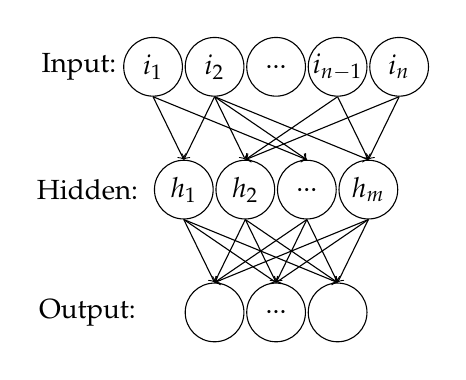
\begin{tikzpicture}
		[ plain/.style={ draw=none, fill=none, }, remember picture, net/.style={ matrix of nodes, nodes={ draw, circle,
			inner sep=7.5pt
			},
		  nodes in empty cells,
		  column sep=-10.5pt,
		  row sep=0.8cm
		  }
		]
	%\draw[help lines] (-3cm,-6cm) grid (6cm,3cm);
	\matrix[net] (mat)
		{
				  & |[plain]| &           & |[plain]|  &           & |[plain]| &           &  |[plain]|      &               \\
		|[plain]| &           & |[plain]| &            & |[plain]| &           & |[plain]| &                 & |[plain]|     \\ 
		|[plain]| & |[plain]| &           & |[plain]|  &           & |[plain]| & 	  	   &  |[plain]|      & |[plain]|     \\ 
	  };

	  \node at ($(mat-1-1.west)+(-16pt,0)$) {Input: };
	  \node at ($(mat-2-2.west)+(-24pt,0)$) {Hidden:};
	  \node at ($(mat-3-2.west)+(-24pt,0)$) {Output:};
	  \node at (mat-1-1.base) {$i_1$};
	  \node at (mat-1-3.base) {$i_2$};
	  \node at (mat-1-5.base) {...};
	  \node at (mat-1-7.base) {$i_{n-1}$};
	  \node at (mat-1-9.base) {$i_{n}$};
	  \node at (mat-2-2.base) {$h_1$};
	  \node at (mat-2-4.base) {$h_2$};
	  \node at (mat-2-6.base) {$...$};
	  \node at (mat-2-8.base) {$h_{m}$};
	  \node at (mat-3-5.base) {$...$};

		 \foreach \a in {1,3}{
			\foreach \b in {2,6}{
				\draw[->] (mat-1-\a.south) -- (mat-2-\b.north);
			 }
		  }
		 \foreach \a in {3,7,9}{
			\foreach \b in {4,8}{
				\draw[->] (mat-1-\a.south) -- (mat-2-\b.north);
			 }
		  }

		 \foreach \c in {2,4,6,8}{
			\foreach \d in {3,5,7}{
				\draw[->] (mat-2-\c.south) -- (mat-3-\d.north);
			}
	 }
\end{tikzpicture}
\caption{General Neural Network}
\label{fig:gnn}
\end{figure}





\subsection{Activation function}

The activation function is one of the critical parts of an ANN. Liu
\cite{liu1996evolutionary} et al. claims that the performance of neural networks with
different activation functions is different, even if they have the same
architecture.  A generalized activation function can be written as

\begin{equation}
	y_i = f_i(\sum_{j=1}^n{w_{ij}x_j - \theta})
\end{equation}

where $y_i$ is the output of the node $i$, $x_j$ is the $j$th input to the
node, and $w_{ij}$ is the connection weight between adjacent nodes $i$ and $j$.
Tab. \ref{tab:transfer_function} displays the most widely adopted activation
functions in the design of an ANN, which is used for the current study.

\begin{table*}[!t]
\centering
\caption{Different Activation Functions}
\label{tab:active_function}
\begin{adjustbox}{width=1\textwidth}
\label{tab:transfer_function}
	\begin{tabular}{lllc}
			\toprule
			Type & Description  & Formula & Range  \\
			\midrule
			Linear   & The output is proportional to the input & $f(x)=cx$                  &  $(-\infty, +\infty)$ \\
			Sigmoid  & A family of S-shaped functions          & $f(x)=\frac{1}{1+e^{-cx}}$ & $(0, 1)$ \\
			tanh     & A family of Hyperbloic functions        & $f(x)=\frac{e^x -e^{-x}}{e^x+e^{-x}}$ & $(0, 1)$ \\
			Gaussian & A coninuous bell-shaped curve           & $f(x)=e^{-x^2}$            & $(0,1)$ \\ 
			ReLU     & A piece-wise function                   & $f(x)= max{0,x}$           & $(0, +\infty)$ \\
			Softplus & A family of S-shaped functions          & $f(x) = ln(1+e^x)$         & $(0, +\infty)$ \\
			\bottomrule
	\end{tabular}
\end{adjustbox}
\end{table*}


\subsection{Weights learning}
The weight training in an ANN is to minimize the error function, such as the
most widely used mean square error function, which calculates the difference
between the desired and the prediction output values averaged overall examples.
Gradient descent algorithm is widely adopted to reduce the value of an error
function, which has been successfully applied in many practical areas. However,
this class of algorithms is plagued by the possible existence of local minima
or ”flat spots” and ”the curse of dimensionality.” One method to overcome this
problem is to adopt a genetic algorithm(GA)


\begin{figure*}
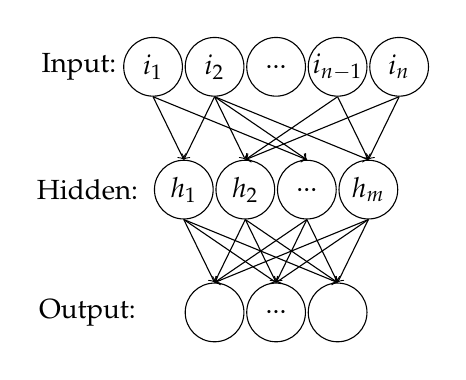
\begin{tikzpicture}
[ plain/.style={ draw=none, fill=none, }, remember picture, net/.style={ matrix of nodes, nodes={ draw, circle,
    inner sep=7.5pt
    },
  nodes in empty cells,
  column sep=-10.5pt,
  row sep=0.8cm
  }
]
%\draw[help lines] (-3cm,-6cm) grid (6cm,3cm);
\matrix[net] (mat)
{
              & |[plain]| &           & |[plain]|  &           & |[plain]| &           &  |[plain]|      &               \\
    |[plain]| &           & |[plain]| &            & |[plain]| &           & |[plain]| &                 & |[plain]|     \\ 
    |[plain]| & |[plain]| &           & |[plain]|  &           & |[plain]| & 	  	   &  |[plain]|      & |[plain]|     \\ 
  };

  \node at ($(mat-1-1.west)+(-16pt,0)$) {Input: };
  \node at ($(mat-2-2.west)+(-24pt,0)$) {Hidden:};
  \node at ($(mat-3-2.west)+(-24pt,0)$) {Output:};
  \node at (mat-1-1.base) {$i_1$};
  \node at (mat-1-3.base) {$i_2$};
  \node at (mat-1-5.base) {...};
  \node at (mat-1-7.base) {$i_{n-1}$};
  \node at (mat-1-9.base) {$i_{n}$};
  \node at (mat-2-2.base) {$h_1$};
  \node at (mat-2-4.base) {$h_2$};
  \node at (mat-2-6.base) {$...$};
  \node at (mat-2-8.base) {$h_{m}$};
  \node at (mat-3-5.base) {$...$};

 \foreach \a in {1,3}{
    \foreach \b in {2,6}{
        \draw[->] (mat-1-\a.south) -- (mat-2-\b.north);
     }
  }
 \foreach \a in {3,7,9}{
    \foreach \b in {4,8}{
        \draw[->] (mat-1-\a.south) -- (mat-2-\b.north);
     }
  }

 \foreach \c in {2,4,6,8}{
    \foreach \d in {3,5,7}{
 		\draw[->] (mat-2-\c.south) -- (mat-3-\d.north);
	}
 }
\end{tikzpicture}
\caption{Neural Network Model}
\end{figure*}



\begin{figure}
\centering
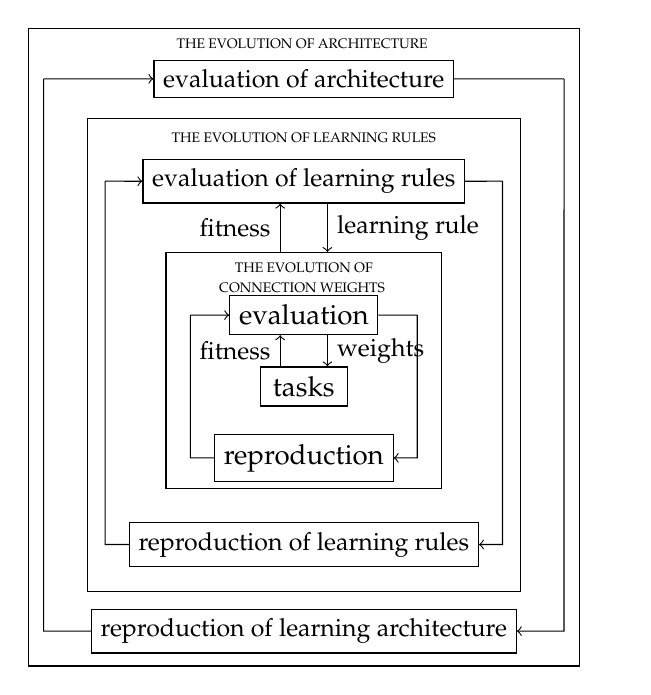
\begin{tikzpicture}
    %\draw[help lines] (-3cm,-6cm) grid (6cm, 6cm);
    \tikzstyle{block} = [rectangle, text centered, draw=black,
    minimum width=1.1cm, minimum height=0.4cm]
    % first level
    \node (evaluation-parent) [block, minimum width=2.4cm, minimum
        height=1.8cm,draw=white] {};
    \node (evaluation) [block] at ($(evaluation-parent.north)$) {evaluation};
    \node (reproduction) [block] at ($(evaluation-parent.south)$) {reproduction};
    \node (tasks) [block, minimum width=1.1cm, minimum height=0.4cm] {tasks};

    \draw[->] ($(evaluation.south)+(0.3cm,0cm)$) --
        ($(tasks.north)+(0.3cm,0cm)$) node[auto=left, pos=0.5] {\small weights}; 
    \draw[<-] ($(evaluation.south)+(-0.3cm,0cm)$) --
        ($(tasks.north)+(-0.3cm,0cm)$) node[auto=right, pos=0.5] {\small fitness}; 

    % get intersection
    \draw[white] (evaluation.west) coordinate (A) -- ++(-1.5cm,0) coordinate (B);
    \draw[white] (reproduction.west) -- ++(-0.3cm,0) coordinate (C) -- ++(0,4cm) coordinate
        (D);
    \draw[black] (reproduction.west) -- ++(-0.3cm,0) -- (intersection cs:
        first line={(A)--(B)}, second line={(C)--(D)}) coordinate (E);
    \draw[->] (E) -- (evaluation.west);

    \draw[white] (evaluation.east) coordinate (E) -- ++(2cm,0) coordinate (F);
    \draw[white] (reproduction.east) -- ++(0.3cm,0) coordinate (G) -- ++(0,4cm) coordinate
        (H);
    \draw[<-] (reproduction.east) -- ++(0.3cm,0) -- (intersection cs:
        first line={(E)--(F)}, second line={(G)--(H)}) coordinate (I);
    \draw (I) -- (evaluation.east);

    % second level
    \node (level2) [block,draw=black, minimum width=3.5cm, minimum height=3.0cm] at
        (0cm,0.2cm) {};
    \node [align=left] at ($(level2.north)+(0,-0.2cm)$) {\tiny THE EVOLUTION
        OF};
    \node [align=left] at ($(level2.north)+(0,-0.45cm)$) {\tiny CONNECTION
            WEIGHTS 
        };
    % third level
    \node (level3-assister) [block, draw=white, minimum width=5cm, minimum
		height=4.6cm] at
        (0, 0.3cm)  {};
    \node (evaluation) [block] at ($(level3-assister.north)$) {\small evaluation of
        learning rules};
    \node (reproduction) [block] at ($(level3-assister.south)$) {\small reproduction of
        learning rules};

    \draw[->] ($(evaluation.south)+(0.3cm,0cm)$) --
        ($(level2.north)+(0.3cm,0cm)$) node[auto=left, pos=0.5] {\small learning
        rule}; 
    \draw[<-] ($(evaluation.south)+(-0.3cm,0cm)$) --
        ($(level2.north)+(-0.3cm,0cm)$) node[auto=right, pos=0.5] {\small fitness}; 

    \draw[white] (evaluation.west) coordinate (A) -- ++(-1.3cm,0) coordinate (B);
    \draw[white] (reproduction.west) -- ++(-0.3cm,0) coordinate (C) -- ++(0,4cm) coordinate
        (D);
    \draw[black] (reproduction.west) -- ++(-0.3cm,0) -- (intersection cs:
        first line={(A)--(B)}, second line={(C)--(D)}) coordinate (E);
    \draw[->] (E) -- (evaluation.west);

    \draw[white] (evaluation.east) coordinate (E) -- ++(2cm,0) coordinate (F);
    \draw[white] (reproduction.east) -- ++(0.3cm,0) coordinate (G) -- ++(0,4cm) coordinate
        (H);
    \draw[<-] (reproduction.east) -- ++(0.3cm,0) -- (intersection cs:
        first line={(E)--(F)}, second line={(G)--(H)}) coordinate (I);
    \draw (I) -- (evaluation.east);
   % fourth level
    \node (level4) [block, draw=black, minimum width=5.5cm, minimum
        height=6.0cm] at
        (0, 0.4cm)  {};
    \node [align=left] at ($(level4.north)+(0,-0.25cm)$) {\tiny THE EVOLUTION
        OF LEARNING RULES};
    % level five
    \node (level5-assister) [block, draw=white, minimum width=6.4cm, minimum
        height=7.0cm] at
        (0, 0.4cm)  {};
    \node (evaluation) [block] at ($(level5-assister.north)$) {\small evaluation of
        architecture};
    \node (reproduction) [block] at ($(level5-assister.south)$) {\small reproduction of
        learning architecture};

    \draw[white] (evaluation.west) coordinate (A) -- ++(-1.5cm,0) coordinate (B);
    \draw[white] (reproduction.west) -- ++(-0.6cm,0) coordinate (C) -- ++(0,4cm) coordinate
        (D);
    \draw[black] (reproduction.west) -- ++(-0.6cm,0) -- (intersection cs:
        first line={(A)--(B)}, second line={(C)--(D)}) coordinate (E);
    \draw[->] (E) -- (evaluation.west);

    \draw[white] (evaluation.east) coordinate (E) -- ++(2cm,0) coordinate (F);
    \draw[white] (reproduction.east) -- ++(0.6cm,0) coordinate (G) -- ++(0,4cm) coordinate
        (H);
    \draw[<-] (reproduction.east) -- ++(0.6cm,0) -- (intersection cs:
        first line={(E)--(F)}, second line={(G)--(H)}) coordinate (I);
    \draw (I) -- (evaluation.east);
    % level 6
    \node (level6) [block, minimum width=7.0cm, minimum
        height=8.1cm] at
        (0, 0.5cm)  {};
    \node [align=left] at ($(level6.north)+(0,-0.2cm)$) {\tiny THE EVOLUTION OF
            ARCHITECTURE
        };
\end{tikzpicture}
\caption{Genetic algorithm and artificial neural network}
\end{figure}


\section{Experiment}
We applied this search strategy to dataset generated by the classic lamination
theory and failure theories. In this dataset, sixtheen attribues and two actual
values are given.

\subsection{Dataset Preparation}
Equation \ref{equ:stress-strain} takes an analytical approach to model the
relationship between stress and strain. We sample this function to yield 14000 points
uniformly distributed over the domain space.

The range of in-plane loading is from 0 to 120; the range of fiber orientation $\theta$ is from
-90 to 90; ply thickness $t$ is 1.27mm, number of plies range $N$ is from 4 to 120;
Three different material is used in this experiment, as shown in table \ref{tab:mat}.
Figure \ref{tab:traing-data} shows part of the training data.

In order to speeds up the learning and accerlate convergence, the input
atttributes of the data set are rescaled to between 0 and 1.0 by a linear function.

\begin{table}	
\label{tab:traing-data}
		\resizebox{\textwidth}{!}{
	\begin{tabular}{cccc|cc}
		\toprule
		\multicolumn{4}{c}{\textbf{Input}} &  \multicolumn{2}{c}{\textbf{Output}} \\
		\midrule
		Load  &  \makecell{Laminate \\ Structure }  & \makecell{Material \\ Property} & \makecell{Failure \\  Property}  & MS & Tsai-Wu \\
		\midrule

		-70,-10,-40,  & 90,-90,4,1.27, & 38.6,8.27,0.26,4.14,  & 1062.0,610.0,31,118,72,  & 0.0102, & 0.0086 \\
		-10,10,0,     & -86,86,80,1.27,& 181.0,10.3,0.28,7.17, & 1500.0,1500.0,40,246,68, & 0.4026, & 2.5120 \\
		-70,-50,80,   & -38,38,4,1.27, & 116.6,7.67,0.27,4.173,& 2062.0,1701.0,70,240,105,& 0.0080, & 0.0325 \\
		-70,80,-40,   & 90,-90,48,1.27,& 38.6,8.27,0.26,4.14,  & 1062.0,610.0,31,118,72,  & 0.0218, & 0.1028 \\
		-20,-30,0,    & -86,86,60,1.27,& 181.0,10.3,0.28,7.17, & 1500.0,1500.0,40,246,68, & 0.6481, & 0.9512 \\
		0,-40,0,      & 74,-74,168,1.27,& 181.0,10.3,0.28,7.17,& 1500.0,1500.0,40,246,68, & 1.3110, & 3.9619 \\
		\bottomrule
		\end{tabular}
	}
\end{table}

\begin{table*}[ht]
\caption{Comparison of the carbon/epoxy, graphite/epoxy, and glass/epoxy properties}
\centering
\begin{adjustbox}{width=1\textwidth}
\label{tab:mat}
\begin{tabular}{cccccc}
\toprule
Property								   & Symbol				  & Unit  &  Carbon/Epoxy&  Graphite/Epoxy  &  Glass/Epoxy   \\
\midrule
Longitudinal elastic modulus			   & $E_1$				  & GPa   &  116.6       &  181             &  38.6           \\
Traverse elastic modulus				   & $E_2$				  & GPa   &  7.67        &  10.3            &  8.27           \\
Major Poisson's ratio					   & $v_{12}$			  &       &  0.27        &  0.28            &  0.26           \\
Shear modulus							   & $G_{12}$			  & GPa   &  4.17        &  7.17            &  4.14           \\
Ultimate longitudinal tensile strength     & $(\sigma_1^T)_{ult}$ & MP    &  2062        &  1500            &  1062            \\
Ultimate longitudinal compressive strength & $(\sigma_1^C)_{ult}$ & MP    &  1701        &  1500            &  610             \\
Ultimate transverse tensile strength       & $(\sigma_2^T)_{ult}$ & MPa   &  70          &  40              &  31              \\
Ultimate transverse compressive strength   & $(\sigma_2^C)_{ult}$ & MPa   &  240         &  246             &  118              \\
Ultimate in-plane shear strength           & $(\tau_{12})_{ult}$  & MPa   &  105         &  68              &  72               \\
Density                                    & $\rho$               & $g/cm^3$ &  1.605    &  1.590           &  1.903               \\
Cost                                       &                      &       &  8           &  2.5             &  1               \\
\bottomrule
\end{tabular}
\end{adjustbox}
\end{table*}


\begin{figure}[h!]
	\centering
	\begin{subfigure}[b]{1.0\linewidth}
		\centering
		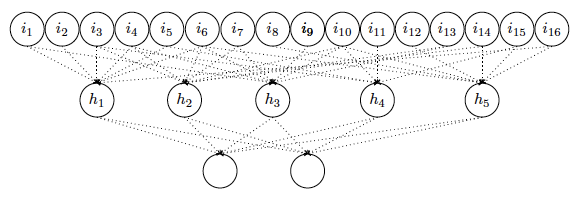
\includegraphics[width=0.8\textwidth]{./a0_figure_ann_for_clt_architecture_example1.png}
		\caption{Parent 1}
		\label{fig:p1}
	\end{subfigure}
	\newline
	\begin{subfigure}[b]{1.0\linewidth}
		\centering
		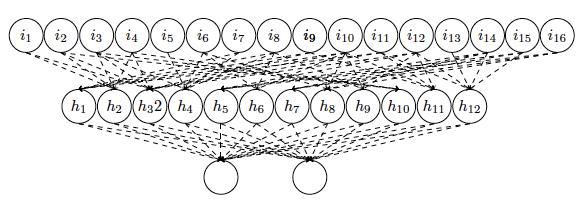
\includegraphics[width=0.8\textwidth]{./a0_figure_ann_for_clt_architecture_example2.png}
		\caption{Parent 2}
		\label{fig:p2}
	\end{subfigure}
	\newline
	\begin{subfigure}[b]{1.0\linewidth}
		\centering
		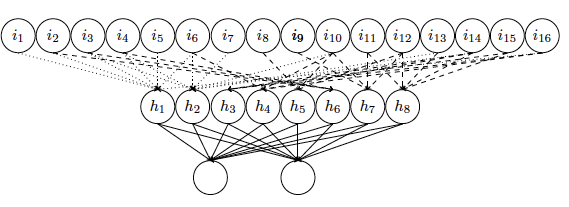
\includegraphics[width=0.8\textwidth]{./a0_figure_ann_for_clt_architecture_child.png}
		\caption{Child}
		\label{fig:child}
	\end{subfigure}
	\caption{Search Operation}
	\label{fig:search}
\end{figure}

%\begin{figure*}
\centering
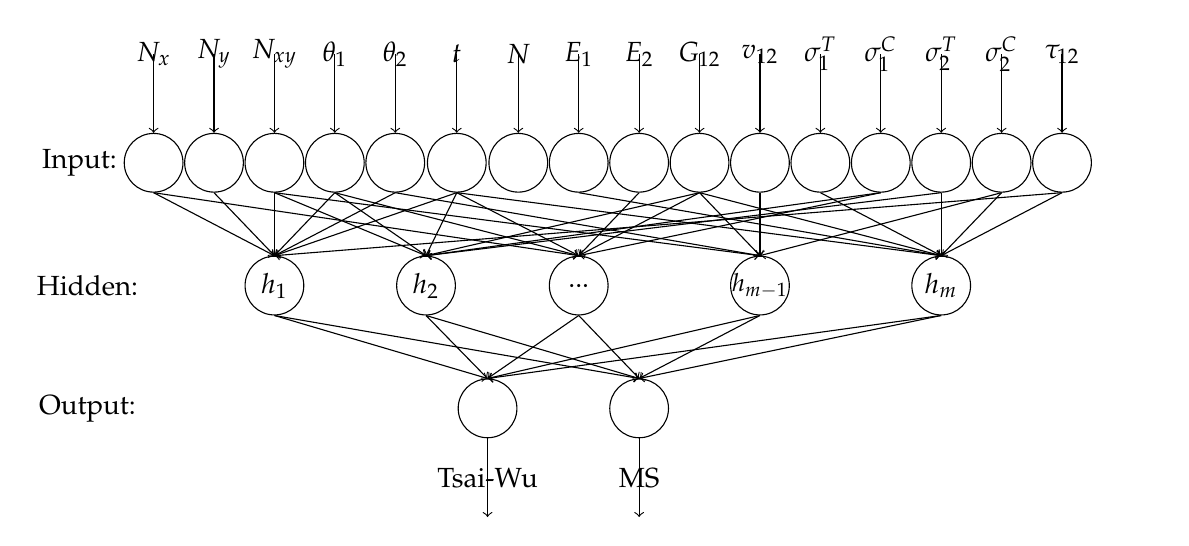
\begin{tikzpicture}
[ p/.style={ draw=none, fill=none, }, remember picture, 
  net/.style={ matrix of nodes, nodes={ draw, circle, inner sep=7.5pt },
  nodes in empty cells,
  column sep=-10.5pt,
  row sep=0.8cm
  }
]
%\draw[help lines] (-3cm,-6cm) grid (6cm,3cm);
\matrix[net] (mat)
{
	  & |[p]| &  & |[p]| &  & |[p]| &  & |[p]| &  & |[p]| &  & |[p]| &  & |[p]| &  & |[p]| &  &
	    |[p]| &  & |[p]| &  & |[p]| &  & |[p]| &  & |[p]| &  & |[p]| &  & |[p]| &  & |[p]|    \\
 |[p]| & |[p]| & |[p]| &  |[p]| &        & |[p]| & |[p]| & |[p]| &|[p]| &       & |[p]| &  |[p]| & |[p]| &
 |[p]| &       & |[p]| &  |[p]| &  |[p]| & |[p]| & |[p]| &       &|[p]| & |[p]| & |[p]| & |[p]|
	   & |[p]| &       &  |[p]| &  |[p]| & |[p]| & |[p]| & |[p]| &|[p]| \\ 
 |[p]| &  |[p]| & |[p]|  &  |[p]| & |[p]|  &  |[p]| &  |[p]| &  |[p]| & |[p]| & |[p]| & |[p]| &       & |[p]|
	   &  |[p]| & |[p]|  &  |[p]| &        &  |[p]| &  |[p]| &  |[p]| & |[p]| & |[p]| & |[p]| & |[p]| &     |[p]|
	   &  |[p]| & |[p]|  &  |[p]| & |[p]|  &  |[p]| &  |[p]| &  |[p]| \\ 
  };
  \draw[<-] (mat-1-1.north) --  ++(0,1) node {$N_x$};
  \draw[<-] (mat-1-3.north) --  ++(0,1) node {$N_y$};
  \draw[<-] (mat-1-5.north) --  ++(0,1) node {$N_{xy}$};
  \draw[<-] (mat-1-7.north) --  ++(0,1) node {$\theta_1$};
  \draw[<-] (mat-1-9.north) --  ++(0,1) node {$\theta_2$};
  \draw[<-] (mat-1-11.north) --  ++(0,1) node {$t$};
  \draw[<-] (mat-1-13.north) --  ++(0,1) node {$N$};
  \draw[<-] (mat-1-15.north) --  ++(0,1) node {$E_1$};
  \draw[<-] (mat-1-17.north) --  ++(0,1) node {$E_2$};
  \draw[<-] (mat-1-19.north) --  ++(0,1) node {$G_{12}$};
  \draw[<-] (mat-1-21.north) --  ++(0,1) node {$v_{12}$};
  \draw[<-] (mat-1-23.north) --  ++(0,1) node {$\sigma_1^T$};
  \draw[<-] (mat-1-25.north) --  ++(0,1) node {$\sigma_1^C$};
  \draw[<-] (mat-1-27.north) --  ++(0,1) node {$\sigma_2^T$};
  \draw[<-] (mat-1-29.north) --  ++(0,1) node {$\sigma_2^C$};
  \draw[<-] (mat-1-31.north) --  ++(0,1) node {$\tau_{12}$};
  \draw[->] (mat-3-12.south) --  ++(0,-1) node[pos=0.5, swap] {Tsai-Wu};
  \draw[->] (mat-3-17.south) --  ++(0,-1) node[pos=0.5, swap] {MS};
  \node at ($(mat-1-1.west)+(-16pt,0)$) {Input: };
  \node at ($(mat-2-2.west)+(-24pt,0)$) {Hidden:};
  \node at ($(mat-3-2.west)+(-24pt,0)$) {Output:};
  \node at (mat-2-5.base) {$h_1$};
  \node at (mat-2-10.base) {$h_2$};
  \node at (mat-2-15.base) {$...$};
  \node at (mat-2-21.base) {\small{$h_{m-1}$}};
  \node at (mat-2-27.base) {$h_{m}$};
 \foreach \a in {1,3,5,7,9,11,31}{
        \draw[->] (mat-1-\a.south) -- (mat-2-5.north);
     }
 \foreach \a in {5,7,11,19,25,27}{
        \draw[->] (mat-1-\a.south) -- (mat-2-10.north);
     }
 \foreach \a in {1,7,11,17,19,25}{
        \draw[->] (mat-1-\a.south) -- (mat-2-15.north);
     }
 \foreach \a in {5,9,19,21,29}{
        \draw[->] (mat-1-\a.south) -- (mat-2-21.north);
     }
 \foreach \a in {11,15,19,23,27,29,31}{
        \draw[->] (mat-1-\a.south) -- (mat-2-27.north);
     }
 \foreach \c in {5,10,15,21,27}{
    \foreach \d in {12,17}{
 		\draw[->] (mat-2-\c.south) -- (mat-3-\d.north);
	}
 }
\end{tikzpicture}
\caption{Neural Network Model}
\end{figure*}



The inputs of the neural network is consist of four parts: in-plane loading
$N_x$, $N_y$, and $N_{xy}$, design parameters of laminate, two distinct fiber
orientation angle $\theta_1$ and $\theta_2$, ply thickness $t$, total number of
plies $N$; five engineering constants of composite materials, $E_1$, $E_2$, ;
five strength parameters of a unidirectional lamina. There are two outputs in
the neural network, safety factors for MS theory and Tsai-Wu theory, respectively.

\begin{figure}
\centering
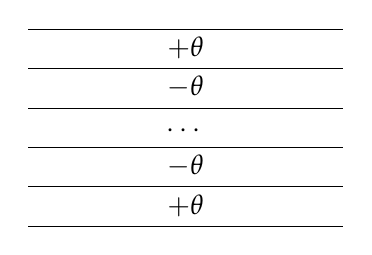
\begin{tikzpicture}
	\draw (0,0) -- (4,0);
	\draw (0,-0.5) -- (4,-0.5) node[midway, above] {$\mathit{+}\theta$};
	\draw (0,-1) -- (4,-1) node[midway, above] {$\mathit{-}\theta$} ;
	\draw (0,-1.5) -- (4,-1.5) node[midway, above] {$\cdots$};
	\draw (0,-2) -- (4,-2) node[midway, above] {$\mathit{-}\theta$};
	\draw (0,-2.5) -- (4,-2.5) node[midway, above] {$\mathit{+}\theta$};
\end{tikzpicture}
\caption{Model for Angle ply laminate}
\end{figure}






%\section{Conclusion}
We review the use of genetic algorithms and artificial neural networks as an
alternative approach for calculating the strength ratio of an angle ply
laminate under in-plane loading, traditionally, which is obtained through CLT,
and corresponding failure theories, such as Maximum stress theory and Tsai-wu
failure theory. To obtain optimal architecture, we propose a two-layer ANN
framework and four levels of evolution on the design of ANN.  It was
demonstrated that ANN is an efficient and simple tool to compute the strength
ratio, instead of the complex analytical mathematical model. Our findings
underline the practical applicability of ANN on the analysis of composite
material.  



\section{Acknowledgment}
The work has partly been supported by the work supported by China Scholarship
Council(CSC) under grant no. 201806630112


 
% Chapter Template

\chapter{Approximation of CLT Based on Artificial Neural Network} % Main chapter title

\label{Chapter5} % Change X to a consecutive number; for referencing this chapter elsewhere, use \ref{ChapterX}

%----------------------------------------------------------------------------------------
%	SECTION 1
%----------------------------------------------------------------------------------------

\section{Neural Network Design}
\subsection{Architecture}

\begin{figure}
	\begin{center}
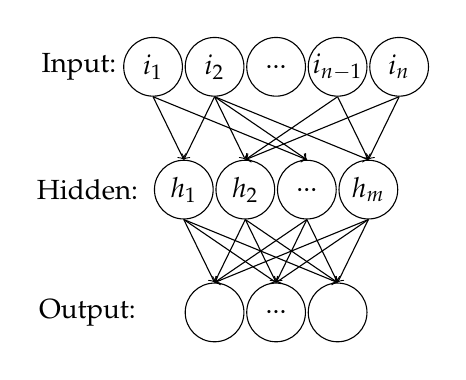
\begin{tikzpicture}
[ plain/.style={ draw=none, fill=none, }, remember picture, net/.style={ matrix of nodes, nodes={ draw, circle,
    inner sep=7.5pt
    },
  nodes in empty cells,
  column sep=-10.5pt,
  row sep=0.8cm
  }
]
%\draw[help lines] (-3cm,-6cm) grid (6cm,3cm);
\matrix[net] (mat)
{
              & |[plain]| &           & |[plain]|  &           & |[plain]| &           &  |[plain]|      &               \\
    |[plain]| &           & |[plain]| &            & |[plain]| &           & |[plain]| &                 & |[plain]|     \\ 
    |[plain]| & |[plain]| &           & |[plain]|  &           & |[plain]| & 	  	   &  |[plain]|      & |[plain]|     \\ 
  };

  \node at ($(mat-1-1.west)+(-16pt,0)$) {Input: };
  \node at ($(mat-2-2.west)+(-24pt,0)$) {Hidden:};
  \node at ($(mat-3-2.west)+(-24pt,0)$) {Output:};
  \node at (mat-1-1.base) {$i_1$};
  \node at (mat-1-3.base) {$i_2$};
  \node at (mat-1-5.base) {...};
  \node at (mat-1-7.base) {$i_{n-1}$};
  \node at (mat-1-9.base) {$i_{n}$};
  \node at (mat-2-2.base) {$h_1$};
  \node at (mat-2-4.base) {$h_2$};
  \node at (mat-2-6.base) {$...$};
  \node at (mat-2-8.base) {$h_{m}$};
  \node at (mat-3-5.base) {$...$};

 \foreach \a in {1,3}{
    \foreach \b in {2,6}{
        \draw[->] (mat-1-\a.south) -- (mat-2-\b.north);
     }
  }
 \foreach \a in {3,7,9}{
    \foreach \b in {4,8}{
        \draw[->] (mat-1-\a.south) -- (mat-2-\b.north);
     }
  }

 \foreach \c in {2,4,6,8}{
    \foreach \d in {3,5,7}{
 		\draw[->] (mat-2-\c.south) -- (mat-3-\d.north);
	}
 }
\end{tikzpicture}
\caption{Neural Network Model}
\end{center}
\end{figure}

\begin{figure*}
\centering
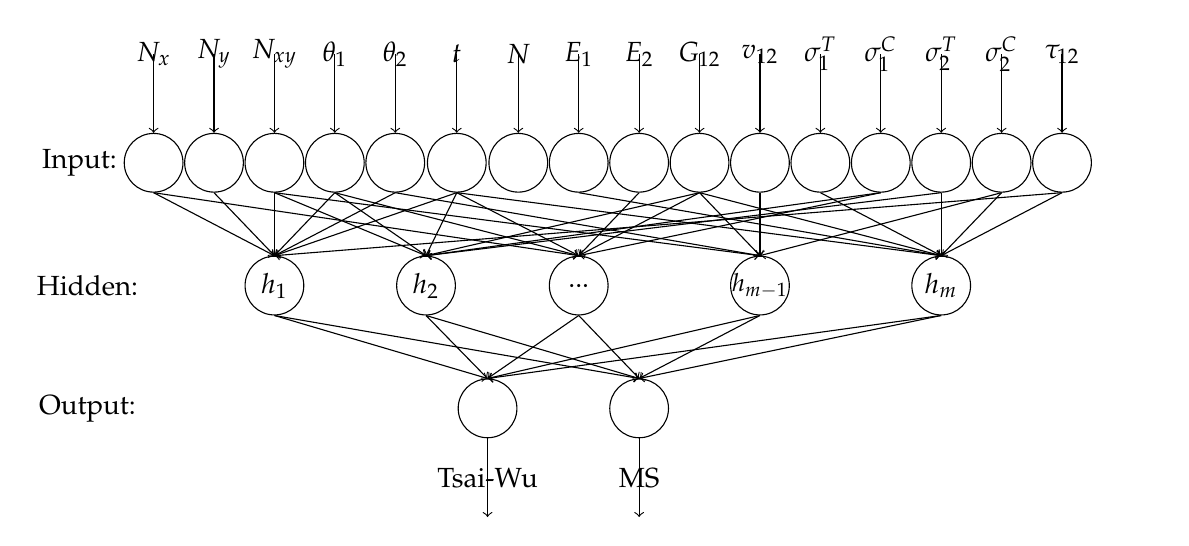
\begin{tikzpicture}
[ p/.style={ draw=none, fill=none, }, remember picture, 
  net/.style={ matrix of nodes, nodes={ draw, circle, inner sep=7.5pt },
  nodes in empty cells,
  column sep=-10.5pt,
  row sep=0.8cm
  }
]
%\draw[help lines] (-3cm,-6cm) grid (6cm,3cm);
\matrix[net] (mat)
{
	  & |[p]| &  & |[p]| &  & |[p]| &  & |[p]| &  & |[p]| &  & |[p]| &  & |[p]| &  & |[p]| &  &
	    |[p]| &  & |[p]| &  & |[p]| &  & |[p]| &  & |[p]| &  & |[p]| &  & |[p]| &  & |[p]|    \\
 |[p]| & |[p]| & |[p]| &  |[p]| &        & |[p]| & |[p]| & |[p]| &|[p]| &       & |[p]| &  |[p]| & |[p]| &
 |[p]| &       & |[p]| &  |[p]| &  |[p]| & |[p]| & |[p]| &       &|[p]| & |[p]| & |[p]| & |[p]|
	   & |[p]| &       &  |[p]| &  |[p]| & |[p]| & |[p]| & |[p]| &|[p]| \\ 
 |[p]| &  |[p]| & |[p]|  &  |[p]| & |[p]|  &  |[p]| &  |[p]| &  |[p]| & |[p]| & |[p]| & |[p]| &       & |[p]|
	   &  |[p]| & |[p]|  &  |[p]| &        &  |[p]| &  |[p]| &  |[p]| & |[p]| & |[p]| & |[p]| & |[p]| &     |[p]|
	   &  |[p]| & |[p]|  &  |[p]| & |[p]|  &  |[p]| &  |[p]| &  |[p]| \\ 
  };
  \draw[<-] (mat-1-1.north) --  ++(0,1) node {$N_x$};
  \draw[<-] (mat-1-3.north) --  ++(0,1) node {$N_y$};
  \draw[<-] (mat-1-5.north) --  ++(0,1) node {$N_{xy}$};
  \draw[<-] (mat-1-7.north) --  ++(0,1) node {$\theta_1$};
  \draw[<-] (mat-1-9.north) --  ++(0,1) node {$\theta_2$};
  \draw[<-] (mat-1-11.north) --  ++(0,1) node {$t$};
  \draw[<-] (mat-1-13.north) --  ++(0,1) node {$N$};
  \draw[<-] (mat-1-15.north) --  ++(0,1) node {$E_1$};
  \draw[<-] (mat-1-17.north) --  ++(0,1) node {$E_2$};
  \draw[<-] (mat-1-19.north) --  ++(0,1) node {$G_{12}$};
  \draw[<-] (mat-1-21.north) --  ++(0,1) node {$v_{12}$};
  \draw[<-] (mat-1-23.north) --  ++(0,1) node {$\sigma_1^T$};
  \draw[<-] (mat-1-25.north) --  ++(0,1) node {$\sigma_1^C$};
  \draw[<-] (mat-1-27.north) --  ++(0,1) node {$\sigma_2^T$};
  \draw[<-] (mat-1-29.north) --  ++(0,1) node {$\sigma_2^C$};
  \draw[<-] (mat-1-31.north) --  ++(0,1) node {$\tau_{12}$};
  \draw[->] (mat-3-12.south) --  ++(0,-1) node[pos=0.5, swap] {Tsai-Wu};
  \draw[->] (mat-3-17.south) --  ++(0,-1) node[pos=0.5, swap] {MS};
  \node at ($(mat-1-1.west)+(-16pt,0)$) {Input: };
  \node at ($(mat-2-2.west)+(-24pt,0)$) {Hidden:};
  \node at ($(mat-3-2.west)+(-24pt,0)$) {Output:};
  \node at (mat-2-5.base) {$h_1$};
  \node at (mat-2-10.base) {$h_2$};
  \node at (mat-2-15.base) {$...$};
  \node at (mat-2-21.base) {\small{$h_{m-1}$}};
  \node at (mat-2-27.base) {$h_{m}$};
 \foreach \a in {1,3,5,7,9,11,31}{
        \draw[->] (mat-1-\a.south) -- (mat-2-5.north);
     }
 \foreach \a in {5,7,11,19,25,27}{
        \draw[->] (mat-1-\a.south) -- (mat-2-10.north);
     }
 \foreach \a in {1,7,11,17,19,25}{
        \draw[->] (mat-1-\a.south) -- (mat-2-15.north);
     }
 \foreach \a in {5,9,19,21,29}{
        \draw[->] (mat-1-\a.south) -- (mat-2-21.north);
     }
 \foreach \a in {11,15,19,23,27,29,31}{
        \draw[->] (mat-1-\a.south) -- (mat-2-27.north);
     }
 \foreach \c in {5,10,15,21,27}{
    \foreach \d in {12,17}{
 		\draw[->] (mat-2-\c.south) -- (mat-3-\d.north);
	}
 }
\end{tikzpicture}
\caption{Neural Network Model}
\end{figure*}



\subsection{Discussion}
\section{Approximation Framework}
\subsection{Data Preparation}
\subsection{Training}
\subsection{Evaluation}
\subsection{Result and Discussion}
\section{Summary}

 

%----------------------------------------------------------------------------------------
%	THESIS CONTENT - APPENDICES
%----------------------------------------------------------------------------------------

%\appendix % Cue to tell LaTeX that the following "chapters" are Appendices

% Include the appendices of the thesis as separate files from the Appendices folder
% Uncomment the lines as you write the Appendices

%% Appendix A

\chapter{Frequently Asked Questions} % Main appendix title

\label{AppendixA} % For referencing this appendix elsewhere, use \ref{AppendixA}

\section{How do I change the colors of links?}

The color of links can be changed to your liking using:

{\small\verb!\hypersetup{urlcolor=red}!}, or

{\small\verb!\hypersetup{citecolor=green}!}, or

{\small\verb!\hypersetup{allcolor=blue}!}.

\noindent If you want to completely hide the links, you can use:

{\small\verb!\hypersetup{allcolors=.}!}, or even better: 

{\small\verb!\hypersetup{hidelinks}!}.

\noindent If you want to have obvious links in the PDF but not the printed text, use:

{\small\verb!\hypersetup{colorlinks=false}!}.

%\include{Appendices/AppendixB}
%\include{Appendices/AppendixC}

%----------------------------------------------------------------------------------------
%	BIBLIOGRAPHY
%----------------------------------------------------------------------------------------

\printbibliography[heading=bibintoc]

%----------------------------------------------------------------------------------------

\end{document}  
